\documentclass[11pt,a4paper,oneside]{article}
\usepackage[left=2cm, right=1.5cm, top=1.5cm]{geometry}
\usepackage{color}
\usepackage[utf8]{inputenc} % Включаем поддержку UTF8  
\usepackage[russian]{babel}  % Включаем пакет для поддержки русского языка  
\usepackage{graphicx}
\usepackage{enumitem}
\usepackage{float}

\graphicspath{ {./images/} }
\DeclareGraphicsExtensions{.png,.pdf,.jpeg,.jpg}

\DeclareUnicodeCharacter{F7}{$\div$}
\DeclareUnicodeCharacter{3B1}{$\alpha$}
\DeclareUnicodeCharacter{3C0}{$\pi$}
\DeclareUnicodeCharacter{2190}{$\leftarrow$}
\DeclareUnicodeCharacter{2192}{$\rightarrow$}
\DeclareUnicodeCharacter{2191}{$\uparrow$}
\DeclareUnicodeCharacter{221A}{$\sqrt{}$}
\DeclareUnicodeCharacter{2260}{$\neq$}
\DeclareUnicodeCharacter{2A7E}{$\geq$}


\providecommand{\tightlist}{%
    \setlength{\itemsep}{0pt}\setlength{\parskip}{0pt}}

\title{Калькулятор}
\makeindex

\begin{document}
\maketitle
\tableofcontents
\pagebreak

\includegraphics[width=6cm]{calculator}
\section{Логика микрокалькулятора}
ИГОРЬ ДАНИЛОВ, кандидат технических наук

Почему микрокалькулятор называется программируемым? Потому что в его память можно записать программу. Но как это сделать?

Режим ввода программы устанавливается клавишами «F ПРГ». Подобно тому как использование переключателя «Р—Г» не подразумевает совершения конкретных операций, клавиша «ПРГ» тоже лишь задает режим интерпретации вводимой информации. Режим же вычислений (не совсем удачно названный в "Руководстве по эксплуатации" автоматической работой) автоматически устанавливается при включении микрокалькулятора. А если нужно перейти к режиму вычислений после ввода программы, необходимо нажать клавиши «F АВТ».

Итак, включаем микрокалькулятор, нажимаем клавиши «F ПРГ». В правом углу экрана появляются цифры 00. Наш ПМК готов к приему программы.

Программа для ПМК представляет собой набор команд-инструкций, следуя которым машина обрабатывает информацию. Полная совокупность команд вместе с правилами их употребления и толкования образует язык микрокалькулятора. Как известно, учить иностранный язык лучше всего, разбирая написанные на нем несложные тексты. Вот и мы начнем с несложных программ — текстов на языке ПМК.

В предыдущей статье мы рассматривали решение простой физической задачи в режиме вычислений. Теперь для тех же целей напишем программу.

Напомним условие. Брусок массой m = 350 г скользит под действием силы, приложенной к нему под углом а. Ускорение бруска $а=0,3 m/c^{2}$, коэффициент трения $k=0,11$. Ускорение свободного падения принять равным $g=9,8 m/c^{2}$. Найти зависимость силы натяжения нити Т и давления бруска на поверхность N от угла а.

В общем виде решение записывается формулами:

x=cosa; y=sina; z=m/(x+ky);

T=z(a+kg); N=z(gx—ay), уже приведенными к виду, наиболее удобному для программирования.

\begin{tabular}{|c|c|c|c|c|c|}\hline
АДРЕС & КОМАНДА & КОД & АДРЕС & КОМАНДА & КОД \\\hline
00 & Fcos & 1Г & 16 & + & 10 \\\hline
01 & П1 & 41 & 17 & X & 12 \\\hline
02 & FBx & 0 & 18 & с/п & 50 \\\hline
03 & FSin & 1C & 19 & ИПД & БГ \\\hline
04 & П2 & 42 & 20 & ИП1 & Б1 \\\hline
05 & ИПВ & БL & 21 & X & 12 \\\hline
06 & X & 12 & 22 & ИПА & 6- \\\hline
07 & + & 10 & 23 & ИП2 & Б2 \\\hline
08 & ИПС & БС & 24 & X & 12 \\\hline
09 & Х4 & 14 & 25 & - & 11 \\\hline
10 & ÷ & 13 & 25 & ИП3 & БЗ \\\hline
11 & П3 & 43 & 27 & X & 12 \\\hline
12 & ИПВ & БL & 28 & с/п & 50 \\\hline
13 & ИПД & БГ & 29 & БП & 51 \\\hline
14 & X & 12 & 30 & 00 & 00 \\\hline
15 & ИПА & Б- & & & \\\hline
\end{tabular}

\begin{tabular}{|c|c|c|c|c|}\hline
КОМАНДА & \multicolumn{4}{|c|}{ИНДИКАТОР} \\\hline
Fcos & 1Г & & & 01 \\
П1 & 41 & 1Г & & 02 \\
FBX & 0 & 41 & 1Г & 03 \\
Fsin & 1С & 0 & 41 & 04 \\\hline
\end{tabular}

А это — программа. Она записана в трех колонках: первая — адрес команды, вторая — сама команда (клавиши, нажимаемые при вводе), третья — код команды. На втором рисунке в первой колонке — команда, во второй — содержимое экрана после ее ввода. Крайнее слева число — код последней введенной команды, затем коды двух предыдущих и, наконец, последняя пара цифр — адрес команды, которую надо вводить. Нам коды нужны для визуального контроля правильности ввода, для машины же они являются именами, названиями команд. Каждый код — двузначное число, правда, не в десятичной, а в шестнадцатеричной системе счисления. Хранится код каждой введенной команды в ячейке, адрес которой высвечивается на экране перед вводом этой команды.

Но как быть, если при вводе допущена ошибка? Если вы увидели, что код набранной команды не соответствует записанному в третьем столбце программы, то нажмите клавишу ← «ШГ» (шаг назад) и повторите ввод. Например, при вводе программы на экране светятся цифры: 1Г 0 41 04. Значит, при вводе команды по адресу 03 произошла ошибка: вместо синуса введен косинус. Нажимаем «ШГ», на экране: 0 41 1Г 03. Повторяем ввод команды «F sin». Читаем: 1C 0 41 04. Теперь все верно.

Но вот программа введена. Если сравнить ее с последовательностью нажатия клавиш для решения задачи из предыдущего выпуска, то легко убедиться, что программа почти полностью повторяет тот же набор. Те же символы знаков операций (сложение — команды по адресам 07 и 16, вычитание — по адресу 25, умножение — 06, 14, 17, 21 и 24), обращение к функциям (sin — адрес 03, cos — адрес 00), команда перемены местами содержимого регистров X и Y (адрес 09) и вызов содержимого регистра XI в регистр X (адрес 02). Но две команды нам еще не встречались. Это «С/П» (18 и 28) и «БП 00». Последняя команда в отличие от всех предыдущих размещается в двух смежных ячейках (по адресам 29 и 30).

Команда «С/П» (стоп/пуск) используется в программе для прекращения процесса вычислений, останова, как говорят программисты. В нашем случае остановки записаны после вычисления величин Т и N, чтобы можно было считать их значения с индикатора. В режиме вычислений эта команда останавливает либо запускает программу.

Команда "БП 00" (в общем случае — «БПnm», где nm — двузначное число от 00 до 97) читается так: безусловный переход на адрес 00. Она прерывает последовательное выполнение команд, записанных в программе. Следующей после этой команды выполняется та, что записана по адресу 00. У нас она введена для того, чтобы по окончании расчета величин Т и N для заданного угла α передать управление к началу программы, обеспечив тем самым возможность расчета при новом значении угла.

После того как программа введена и записана в память, нужно перевести наш ПМК в режим вычислений. Нажимаем клавиши «F АВТ». Машинка готова считать, но она пока что "не знает" числовых значений величин. На их месте записаны команды «ИП А», «ИП В» и т. д. Величина а должна быть записана в регистр RA, к - в RB, m — в RC, и g — в RД. Но сами они туда не попадут, их надо ввести. После установки режима вычислений набираем на клавиатуре нужное число, затем нажимаем клавиши «П» и номер регистра. Проведем эту работу: «0.3 ПА», «0.11 ПВ», «0.35 ПС», «9.8 ПД». Величины a, k, m и g записаны в соответствующие регистры. Теперь нужно сделать так, чтобы программа начала работать с того адреса, где записана ее первая команда (в нашем случае с нулевого). Нажимаем клавишу «В/О» (воз- врат/очистка). Наконец, нужно ввести переменную величину, значение угла α в градусах в регистр X (проверьте заодно, установлен ли переключатель «Р—Г» в положение «Г»), Набираем на клавиатуре нужное число, для начала 40. Нажим клавиши «С/П» запускает программу на счет. Примерно через 10 с на индикаторе появляется: 5.7639597—01. Первые 8 цифр — мантисса числа, две последние со знаком — порядок
числа. Снова нажимаем "с/п". Секунд через пять считываем второе число: 3.0594998. Если числа на экране другие, значит, при вводе программы допущена ошибка. Простейший путь исправить ее — выключить калькулятор, секунд через десять включить вновь и повторить ввод программы, строго контролируя каждый шаг.

Если же числа совпали, можно продолжать расчеты. Теперь достаточно набирать на клавиатуре значение угла в градусах и нажимать на клавишу «С/П». По результатам можно построить графики. Интересно, например, выяснить, при каком значении угла сила давления бруска на поверхность равна нулю. Правда, точное значение этого угла получить невозможно, зато его можно определить с большой степенью точности. Кстати, почему сила давления меняет знак? Что за смысл в отрицательном давлении? Чтобы ответить на этот вопрос, не обойтись без знания физики. Вот и пример использования ПМК при изучении этой науки.

Но вернемся к самому микрокалькулятору. Когда программа запущена, на экране мелькают цифры. Что происходит в это время внутри ПМК?

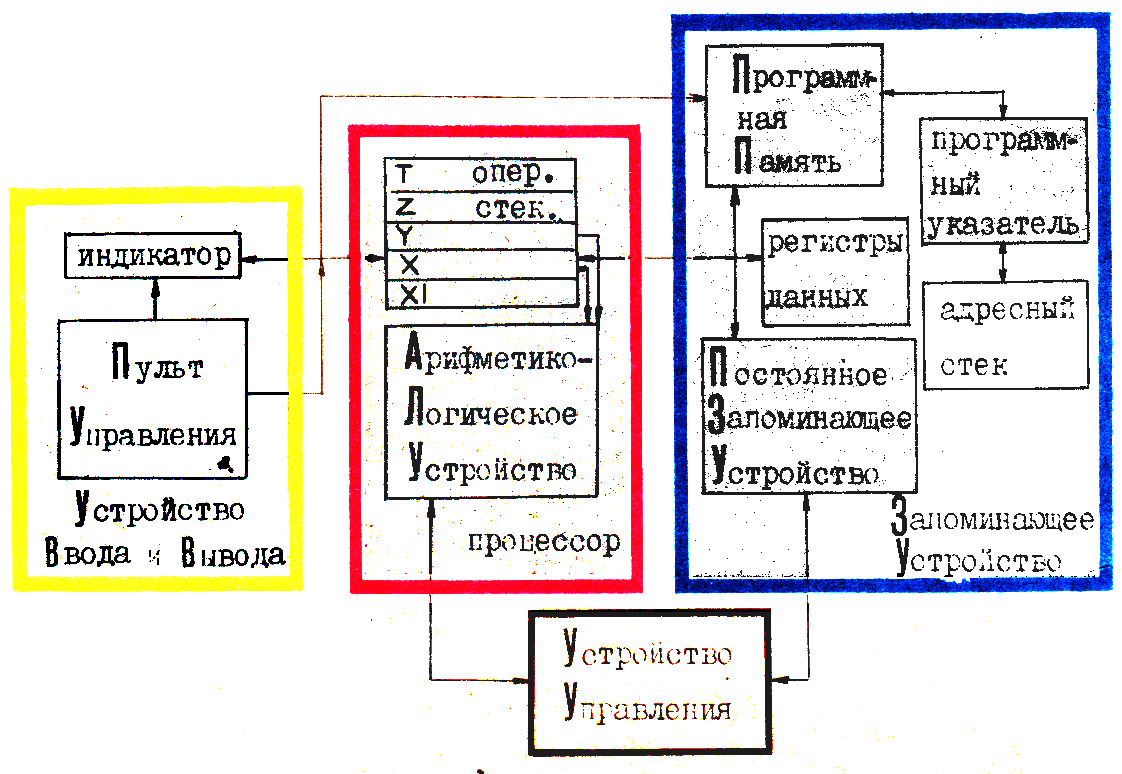
\includegraphics[width=\textwidth]{princip_scheme}

Принципиальная схема микрокалькулятора изображена на рисунке. Основными ее элементами являются устройство ввода и вывода информации (УВВ), устройство преобразования информации (процессор), запоминающее устройство (ЗУ) и устройство управления (УУ).

Устройство ввода и вывода — единственное, которое мы непосредственно видим. Состоит оно из клавиатуры, совмещающей функции устройства ввода и пульта управления, и индикатора. Программа и числа, вводимые с клавиатуры, отображаются на индикаторе. Туда же выводятся результаты вычислений. Индикатор, вообще говоря, — единственное "окно" в память машины, с помощью которого можно получить сведения о ее содержимом.

Команда, введенная с клавиатуры, попадает в запоминающее устройство. Состоит ЗУ из нескольких различных секций: программная память, регистры данных, постоянное запоминающее устройство (ПЗУ), а также программный указатель и адресный стек.

Программная память (ПП) представляет собой набор ячеек, в каждую из которых можно записать один код. Всего таких ячеек 98, нумеруются они двузначными числами  от 00 до 97. Количество ячеек определяет максимальную длину программы, которую можно ввести в память микрокалькулятору. Организована ПП наподобие "колеса обозрения". Адрес текущей ячейки записывается в программном указателе. При вводе команды адрес этот автоматически увеличивается на единицу и "колесо" поворачивается, подготавливая следующую "кабинку" (ячейку) для приема очередного "пассажира" (команды). Содержимое программного указателя можно изменять — с пульта или программным путем (об этом позже). При этом "колесо" может поворачиваться в любую сторону на заданное число позиций. Когда все 98 ячеек программной памяти заполнены, попытка ввести новую команду приводит к повороту "колеса" в начальное положение и команда попадает в первый адрес памяти, естественно стирая его старое содержимое.

Адресный стек состоит из пяти ячеек и используется для запоминания адреса команды, на которую нужно передать управление после окончания работы какой-либо подпрограммы (об использовании подпрограмм будет сказано в одной из следующих статей).

Регистры данных служат для записи и хранения числовой информации. Всего их 14. Таково максимальное количество чисел, которые можно одновременно хранить в памяти ПМК.

Постоянное запоминающее устройство содержит программы, которые, собственно, и организуют процесс вычислений. Эти программы нельзя изменить, они реализованы не программно, а аппаратно, то есть представляют собой совокупность электронных схем. Их нельзя даже прочесть, к ним можно лишь обращаться и получать результаты их работы. Именно программы из ПЗУ подсчитывают значения функций, названия которых записаны на клавиатуре, обеспечивают выполнение арифметических операций.

Выполняет же все операции по программам, хранящимся в ПЗУ, процессор — точнее, арифметическо- логическое устройство (АЛУ), работающее совместно с операционным стеком. В этом стеке 5 регистров: XI, X, Y, Z, Т. Числа движутся по регистрам либо автоматически (при выполнении некоторых операций), либо подчиняясь специальным командам. Подробно движение информации в стековых регистрах будет рассмотрено в одной из следующих статей. Особо важны два регистра: X и Y. Из них АЛУ черпает числовую информацию для выполнения двухместных операций: сложения, вычитания, умножения, деления и возведения в степень. Одноместные операции: извлечение квадратного корня, возведение в квадрат, вычисление тригонометрических функций и т. д. — производятся над содержимым регистра X.

В соответствии с кодом команды АЛУ вырабатывает результат операции и помещает его в регистр X. На экране отображается лишь содержимое этого регистра. Так что на индикаторе во время работы ПМК мелькают промежуточные результаты вычислений, появляющиеся в регистре X.

Наконец, устройство управления обеспечивает совместную работу всех блоков ПМК.

Зная функции отдельных элементов микрокалькулятора, проследим теперь полный цикл его работы при выполнении программы. Предположим, что она уже введена в память, установлен режим вычислений и все необходимые числа введены в нужные регистры. Нажимом клавиши «В/О» мы очищаем программный указатель, то есть устанавливаем его содержимое равным нулю. Клавиша, «С/П» запускает программу. Устройство управления считывает команду, адрес которой записан в программ ном указателе. После ее анализа и определения типа операции команда пересылается в АЛУ. По сигналам, поступившим из УУ, процессор вырабатывает результат операции. Затем УУ опрашивает программный указатель и выясняет, какая команда должна выполняться следующей. Потом цикл повторяется. Время выполнения цикла зависит от типа команды и колеблется от десятых долей секунды для команд типа записи и считывания, а также операций типа сложения, до нескольких секунд для вычисления тригонометрических функций. Знание времени выполнения отдельных команд помогает строить более быстродействующие программы.

Теперь подведем итоги.
\begin{enumerate}
\tightlist
\item Микрокалькулятор может работать в двух режимах: 1) ввода и редактирования программ и 2) вычислений. Первый устанавливается клавишами «F ПРГ», второй — «F АВТ». При включении ПМК автоматически устанавливается режим вычислений.
\item Программа для микрокалькулятора состоит из последовательности команд, вводится с клавиатуры и записывается в программную память. Помните, что адрес, который высвечивается при вводе в правом углу индикатора, — это адрес следующей вводимой команды.
\item Порядок работы с программой.
\begin{enumerate}[label=\arabic*)]
\item Установить режим «F ПРГ».
\item Ввести программу.
\item Перейти в режим вычислений «F АВТ».
\item Ввести постоянные в адресуемые регистры.
\item Установить начальный адрес считывания программы.
\item Набрать на клавиатуре значение переменного параметра.
\item Запустить программу на счет.
\item Если нужно повторить расчет для другого значения переменного параметра, перейти к пункту 6.
\end{enumerate}
\item Максимальная длина программы — 98 шагов, максимальное количество чисел, которые могут одновременно храниться в памяти, — 14.
\end{enumerate}

\subparagraph{двоичная система}
10 + 10 = 100!
Это не ошибка и не опечатка. Именно такой результат получается, если числа записаны в двоичной системе счисления.

Системой счисления называется способ выражения и записи чисел. Числа записываются в виде последовательности специальных символов. Смысл каждого символа зависит от позиции или разряда, в котором он записан. Количество единиц младшего разряда, объединяемого в одну единицу старшего, называется основанием системы, а символы, используемые для обозначения единиц каждого разряда, — цифрами.

Наиболее употребительна десятичная система. Мы настолько привыкли к этой системе, что "раскрываем" любое число не задумываясь. Например, $512 = 2 + 1 * 10 + 5*10^{2}$. Эта система представляется нам столь же естественной, как ребенку — родной язык. Но любая система счисления столь же естественна, как и любой язык. В вычислительной технике используются двоичная, восьмеричная и шестнадцатеричная система. Двоичная — самая простая и наиболее удобная для технической реализации. Цифр в ней всего две — 0 и 1. Когда в разряде (а называется двоичный разряд "бит"; несколько двоичных разрядов, чаще всего восемь, объединяются в "байт" — величину, с которой ЭВМ работает как с одним целым) накапливаются две единицы, то они заменяются единицей старшего разряда. Число $2_{10}$ (цифрой внизу обозначается основание системы) в двоичной системе записывается как $10_{2}$. Вообще любое число, записанное в n-ричной системе, переводится в десятичную очень просто. К последней n-ричной цифре прибавляется предпоследняя, умноженная на n, затем стоящая перед ней и умноженная на $n^{2}$, и т. д. Скажем, двоичное число $101_{2} = 1+0*2 + 1*2^{2} = 5_{10}$. Привлекательность двоичной системы, как уже говорилось, — в простоте технической реализации. Каждый разряд — это некоторое устройство, которое может находиться всего в двух состояниях.

В микрокалькуляторе для размещения одного символа кода отводится "тетрада" — четыре двоичных разряда. Легко подсчитать максимальное число, которое можно записать таким образом: $1111_{2} = 1 + 1 * 2 + 1 * 2^{2} + 1 * 2^{3} = 15_{10}$. Значит, коды должны изображаться числами в шестнадцатеричной системе. Так как десятичных знаков для изображения таких чисел не хватает, приходится "выдумывать" дополнительные символы. В ПМК число 10 изображается символом «—», 11 — «L», 12 — «С», 13 — «Г», 14 — «Е». "Цифра" 15 в обозначениях кодов не используется.

\section{Язык микрокалькулятора}
ИГОРЬ ДАНИЛОВ,
кандидат технических наук

Язык микрокалькулятора (как и любой язык) представляет собой набор символов, а также правил, определяющих, как с помощью этих символов писать и понимать написанное.

Правда, в отличие, скажем, от русского языка, где слова расчленяются на буквы, изменяются при склонении или спряжении, язык микрокалькулятора напоминает скорее китайский либо японский. Его "словарь" состоит из несклоняемых слов-иероглифов, и лишь порядком их следования определяется смысл текстов — программ для ПМК. Каждый из иероглифов — это имя команды: надпись на клавише или над ней (а в нижнем ряду — и под клавишей). Клавиши К и F самостоятельной роли не играют: по своему действию они подобны переключателю регистров пишущей машинки. Если требуется иероглиф, начертанный на клавише, то нужно нажать только ее, если же иероглиф, написанный над клавишей, то предварительно необходимо воспользоваться клавишей F (а в некоторых случаях — клавишей К). Каждая команда, независимо от количества нажимаемых клавиш (а оно для некоторых команд доходит до трех), отображается в памяти и на индикаторе одним двузначным шестнадцатеричным числом — кодом. Исключение составляют команды переходов: после них указывается адрес перехода, поэтому за кодом команды обязательно следует код этого адреса.

Полный набор команд «Электроники БЗ-34» приведен в таблице. Ею могут пользоваться и владельцы микрокалькуляторов «Электроника МК-54» и «Электроника МК-56» — система команд у них та же самая. Различаются лишь некоторые обозначения X → П вместо П, П→X вместо ИП, X ←→У вместо XY и В↑ вместо ↑, а также названия обратных тригонометрических функций — $sin^{-1}$, $cos^{-1}$, $tg^{-1}$ вместо arcsin, arccos, arctg. Смысл же операций и их коды полностью идентичные приведенным в таблице.

Условно всю совокупность команд можно разбить на два класса. К первому относятся команды, используемые в программе; ко второму — команды, предписывающие порядок работы ПМК. Последние вводятся в режиме вычислений; мы рассмотрим их при описании процесса отладки программ.

Первый класс можно подразделить на четыре группы: 1) вычислительные команды; 2) команды обмена информацией; 3) команды управления ходом вычислений; 4) команды, использующие режим косвенной адресации. Последние по своим функциям не отличаются от команд второй и третьей групп, но, поскольку используют иной режим адресации, будут рассмотрены отдельно. Особняком стоит команда К НОП.

К первой группе относятся прежде всего команды арифметических операций: сложение + (код 10), вычитание — (11), умножение X (12) и деление ÷(13). Все они двухместные — работают с содержимым двух регистров стека X и Y, причем при вычитании в X записывается вычитаемое, а при делении — делитель. Результат каждой из арифметических операций заносится в регистр X, прежнее содержимое этого регистра перемещается в XI. То, что было в Y, пропадает, замещаясь числом из регистра Z, а в Z заносится содержимое регистра Т. Но при этом прежнее содержимое регистра Т остается и на своем месте.

Надо сказать, что микрокалькулятор способен работать не со всякими числами. Максимальное не должно превосходить $10^{100}$ (точнее, $9,9999999*10^{99}$), минимальное должно быть не меньше $10^{99}$ — в противном случае вместо нормального восьмиразрядного числа в память и на индикатор запишется "чистый" нуль. Наибольшую осторожность надо соблюдать при умножениях и делениях. Иногда случается, что конечный результат цепочки операций лежит в пределах возможностей ПМК, а на промежуточном этапе возникает аварийная остановка. Её можно избежать, правильно организуя процесс вычислений.

Рассмотрим простой пример. Нужно вычислить значение дроби $a*b/c$, где $а=2*10^{51}$, $b=3*10^{49}$, $с=4*10^{50}$. Легко видеть, что результат ($1,5*10^{50}$) лежит в допустимых пределах. Но если соответствующий фрагмент программы записать так: ИП А, ИП В, X, ИП С, ÷, то есть сначала выполнять умножение (мы считаем, что исходные величины хранятся в одноименных регистрах), то после первого же действия получается число $6*10^{100}$, возникает "аварийный" останов, на экране появляется сообщение ЕГГО.Г и вычисления прекращаются. Если же выполнять сначала деление (например, записать тот же фрагмент так: ИП А, ИП С, ÷, ИП В, X)» то никаких неприятностей не произойдет.

К арифметическим можно отнести и команду (—) (код 0L). Она одноместная, использует только регистр X. При ее выполнении меняется знак числа, находящегося в этом регистре (плюс на минус или наоборот).

Остальные вычислительные команды используются для расчета значений различных функций. Их названия написаны над соответствующими клавишами. Чтобы получить значение какой-либо из них, нужно предварительно нажать клавишу F, но для краткости при описании команд мы ее упоминать не будем.

Какие же функции доступны нашему ПМК? Вот они: извлечение квадратного корня $\sqrt{}$ (код 21);
возведение в квадрат $X^{2}$ (22); получение обратной величины $1/X$ (23); возведение числа 10 в любую степень $10^{x}$ (15) и возведение в степень числа е, основания натуральных логарифмов $e^{x}$ (16); вычисление десятичного и натурального логарифмов lg (17) и ln (18); вычисление тригонометрических функций (аргументы могут быть заданы как в градусах, так и в радианах) sin (1C), cos (1Г), tg (1E), а также обратных тригонометрических функций arcsin (19), arccos (1—) и arctg (1L). Аргумент для каждой из этих функций берется из регистра X, туда же записывается результат, а аргумент после выполнения операции перемещается в XI. Содержимое других регистров не меняется.

Особняком среди команд подобного рода стоит $Х^{y}$ (24) — возведение произвольного числа в любую степень. Возводимое число берется из регистра X, а показатель степени — из Y. После выполнения команды результат, как и обычно, заносится в X, то, что было там прежде, переходит в XI, а вот содержимое Y, как и остальных регистров, остается на месте. Отметим, что эту команду «Электроника БЗ-34» выполняет хуже других: результата приходится ждать долго, да и точность его ниже, чем при выполнении других команд. Так, $2^{2}$, вычисленное по этой команде, "равно" 3,9999996. А вот если использовать команду $X^{2}$, результат равен в точности четырем. Калькуляторы же первых выпусков при выполнении команды $X^{y}$ иногда вообще ошибаются. Так что рекомендуем по возможности ее избегать.

Вычислительные команды способны работать не со всеми возможными числами. Иногда это ограничения чисто математические (нельзя, скажем, извлекать квадратный корень из отрицательного числа или вычислять его логарифм), иногда диктуются возможностями ПМК. Поскольку числа, доступные микрокалькулятору, ограничены по абсолютной величине, то аргументы функций $10^{x}$ и $e^{x}$ не могут превосходить соответственно 99,999999 и 230,25. Не допускаются и отрицательные аргументы, по абсолютной величине превосходящие эти числа. Функция $X^{y}$, независимо от величины показателя, не определена для отрицательных оснований. При вычислении тригонометрических функций запрещается выбирать в качестве аргумента числа, превышающие $10^{1}$ (независимо от того, измеряются ли они в градусах или в радианах).

Напомним, что в микрокалькуляторах типа «Электроника БЗ-34» используется обратная бесскобочная (или польская) запись арифметических выражений. Сначала выписываются аргументы операции, а потом ее символ — например, не аХb, а аbХ; не $\sqrt{c}$, а $c\sqrt{}$.

При составлении программ нужно следить, чтобы перед совершением каждой арифметической операции стек был заполнен так, как требуется для ее выполнения.

\begin{figure}[h]
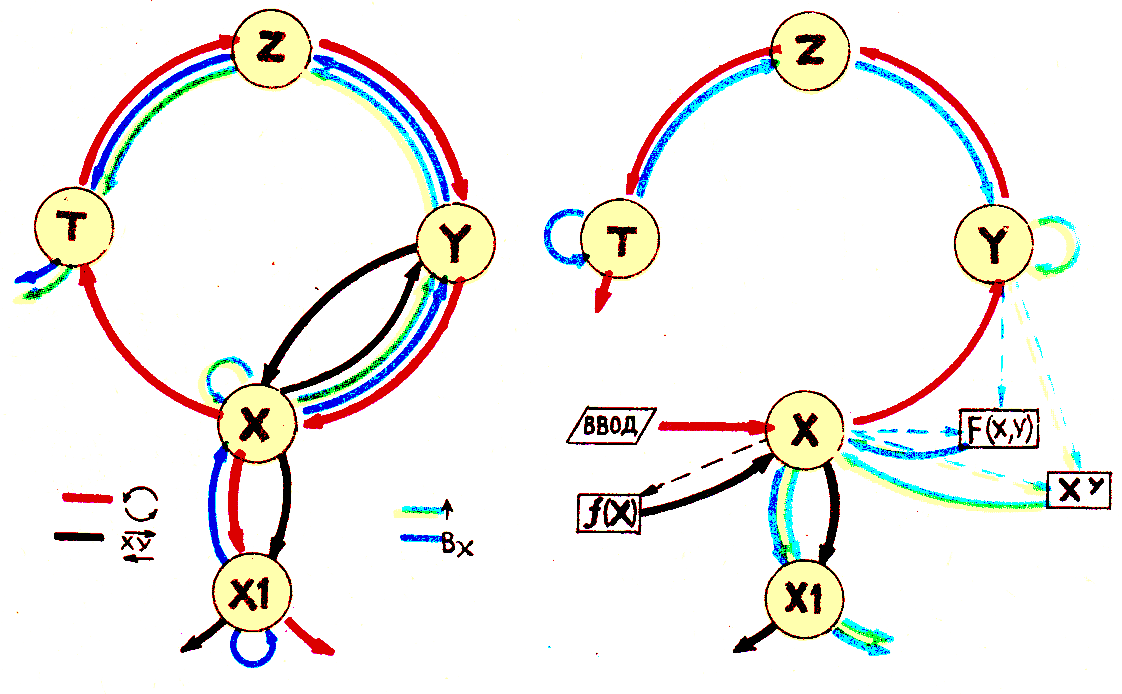
\includegraphics[width=\textwidth]{stack}
\caption{Движение информации по регистрам стена при выполнении команд обмена информацией (слева), ввода и вычислительных операции (справа).}
\end{figure}

Перемещением чисел по регистрам стека и по регистрам данных "заведуют" команды второй группы (команды обмена информацией). Это ↑(ОЕ), F Вх (0), XY (14) и FO (25). Первая из них, ↑ используется чаще всего для разделения вводимых чисел. Она сдвигает числа в стеке "снизу вверх" (см. рис.), сохраняя содержимое регистра X и выбрасывая за пределы стека число, хранившееся в регистре Т. F Bx используется для вызова содержимого регистра предыдущего результата (XI) в регистр X. В остальном ее действие подобно действию предыдущей команды; сдвиг чисел в стеке "снизу вверх" и вытеснение содержимого регистра Т. Команда XY меняет местами содержимое регистров X и Y; при этом число, находившееся в регистре X, дополнительно копируется и в регистре XI, вытесняя его прежнее содержимое. То, что было в остальных регистрах, при этом не меняется. FO совершает круговой обмен: число из регистра X перемещается в Т, содержимое Y передвигается в X, Z — в Y, а Т — в Z. Пропадает при этом только содержимое регистра XI: туда копируется число из X. Движение информации при выполнении всех этих команд отражено на диаграммах.

Есть 14 команд, позволяющих пересылать содержимое регистра X в адресуемые регистры (или регистры данных). Всего их тоже 14. Первые десять обозначаются цифрами от 0 до 9, последние — буквами А, В, С, Д. Для занесения в них информации служат команды: ПО (код 40), П1 (41)... П9 (49). ПА (4—), ПВ (4L), ПС (4С) и ПД (4Г). Каждая из команд требует набора двух клавиш: П и номера регистра (цифры или буквы), но, как мы видим, отображаются они одним кодом — как в памяти, так и на индикаторе. Обратите внимание, что буквы А, В, С и Д написаны под клавишами, но после нажатия клавиши П воспринимаются именно они.

Для вызова информации из адресуемых регистров в регистр X служат команды ИП0 (код 60)... ИП9 (69), ИП А (6—)... ИП Д (6Г). Условно к ним можно отнести и команду Fπ, действие которой заключается в вызове записанного в ПЗУ числа π в регистр X.

В языке микрокалькулятора нет специальных команд ввода. Числа просто набираются на клавиатуре и автоматически заносятся в регистр X. Однако можно хранить числа и в программной памяти. Например, если нужно умножить содержимое регистра 0 на 2, мы пишем обычно: ИП0, 2, X. Теперь при работе программы число 2 вводить не надо — оно занесено в программную память, занимая в ней одну ячейку. Для многозначных чисел такая запись, как правило, нецелесообразна. Например, если мы решим занести в программную память вместо двойки число 2,58, то соответствующий фрагмент программы будет выглядеть так: ИП0, 2, «,», 5, 8, X. Одно число занимает целых четыре ячейки — слишком много! Однако если все адресуемые регистры заняты, а в ПП место есть, то волей-неволей приходится прибегать и к этому способу. Коды цифр совпадают с ними самими (от 00 до 09); кроме них, при вводе чисел в ПП используются символы «,» (код 0—) и ВП (ОС) — ввод порядка. Так, для записи в ПП числа $1,6*10^{-19}$ (заряд электрона в кулонах) нужно ввести команды: 1, «,», 6, ВП, 1, 9, /—/.

Последняя команда этой группы — Сх (код 0Г). Она "стирает" содержимое регистра X (вернее, засылает туда число 0).

Рассмотренных команд достаточно для написания несложных программ, производящих вычисления по последовательным формулам. Однако для многих задач этого набора недостаточно. Даже при решении элементарного квадратного уравнения требуется сначала проверить знак дискриминанта квадратного трехчлена, чтобы знать, вычислять ли действительные корни уравнения, или же действительную и мнимую части корней комплексных. То есть нужно сначала выбрать путь и лишь потом начинать вычисления.

В языке микрокалькулятора имеются средства для проведения подобных операций. Это команды управления программой.

Наиболее часто употребляется команда останова С/П (код 50). Она используется для приостановки процесса вычислений, когда нужно либо прочесть полученный результат, либо ввести с клавиатуры какие-нибудь числа или предписывающие команды. В каждой программе обязательно есть хотя бы одна команда С/П — не может же программа работать бесконечно!

Команда безусловного перехода БП (51) передает управление команде, адрес которой записан сразу после нее. Фактически она занимает в памяти две смежные ячейки: в первой записан код 51, во второй — другое двузначное число, адрес перехода. Так что две цифры подряд,набранные после команды БП, записываются одним кодом — числом от 00 до 97 (напомним, что память ПМК состоит из 98 ячеек, поэтому адресов 98 и 99 попросту нет).

Команды условного перехода тоже передают управление, но лишь при выполнении определенных условий. В качестве условия в этих командах нашего ПМК используется сравнение содержимого регистра X с нулем. Если условие, записанное в команде, выполнено, то управление передается на следующую по порядку команду, в противном случае — по указанному адресу. Например, условный переход х<0, 23 выполняется так. Если число, находящееся в регистре X, меньше нуля, то выполняется команда, следующая за приведенным фрагментом, в противном случае — команда, код которой записан по адресу 23. Команд условного перехода четыре: х<0 (5С), х=0 (5Е), х≠0 (57), х⩾0(59).
Поскольку названия их написаны над клавишами, то перед ними нужно нажимать клавишу F.

Есть среди команд перехода четыре команды, предназначенные для организации циклов — многократного выполнения заданной последовательности команд. Это L0 (код 5Г), L1 (5L), L2 (58) и L3 (5—). Перед каждой из них тоже, естественно, нажимается клавиша F. А после каждой указывается адрес перехода. При обращении к одной из команд организации цикла из содержимого соответствующего (имеющего тот же номер) регистра данных вычитается единица, и, если результат не равен нулю, управление передается по указанному адресу перехода. Если же результат равен нулю, цикл завершается, и выполняется команда, записанная после адреса перехода. Таким образом, заслав в один из первых четырех регистров данных некоторое число n, мы получаем возможность выполнить некоторую часть программы n раз.

Последняя из программ перехода — это ПП (код 53) — переход на подпрограмму. Структура ее такая же, как и у остальных: сначала записывается сама команда, за ней — адрес перехода. Но в отличие от команды БП она не только "безусловно" передает управление по заданному адресу, но и после отработки подпрограммы — а последнюю обязательно завершает команда В/О (возврат/очистка, код 52), — автоматически возвращает программу "на старое место" — к команде, следующей за ПП.

Особняком стоит команда К НОП (код 54), которая набирается двумя клавишами К и НОП. Это — "пустая" команда, она не совершает никаких действий. Употребляется обычно при отладке программ: если выяснится, что одна из команд лишняя, то, чтобы не переписывать остальные, на ее место записывают "пустую" команду.

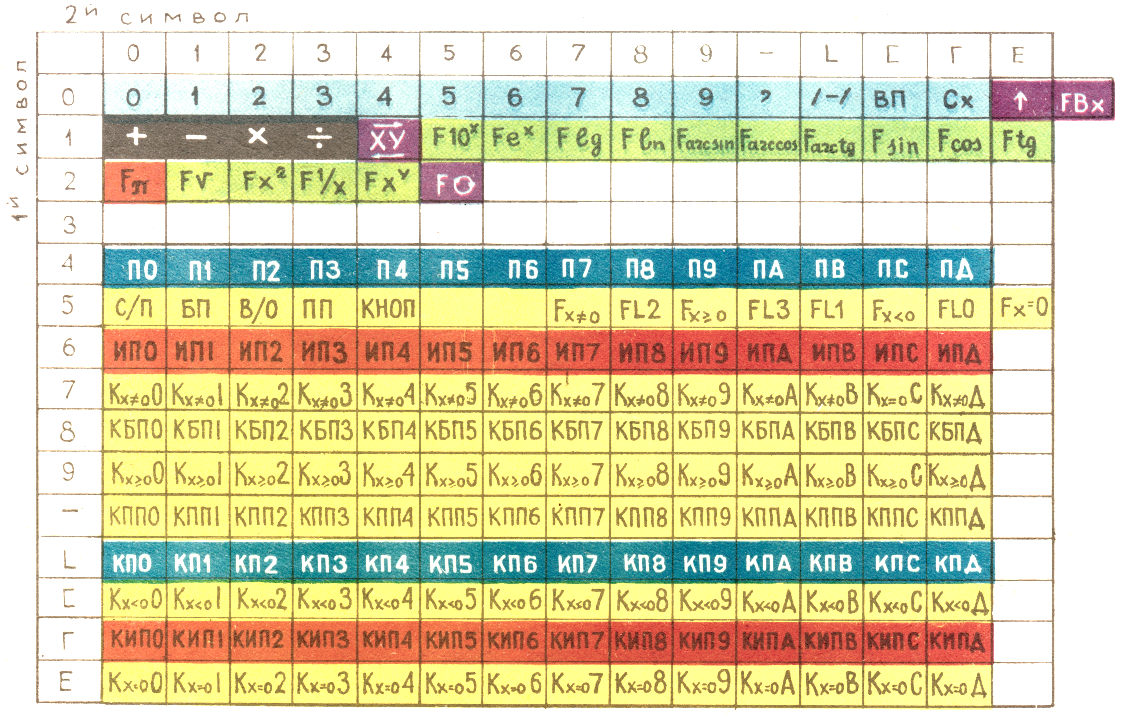
\includegraphics[width=\textwidth]{commands}

Команды косвенной адресации мы рассмотрим позже. Подведем краткие итоги.

\begin{enumerate}
\item Язык микрокалькулятора — это набор команд, имена которых написаны на клавиатуре. Чтобы использовать команды, названия которых даны над клавишами, нужно предварительно нажать клавишу F. Перед командой НОП нужно нажать клавишу К.
\item Каждая вычислительная команда размещается в одной ячейке памяти.
\item Результаты работы вычислительных команд помещаются в регистр X. Исходные данные для одноместных операций черпаются из этого же регистра, а для двухместных — из регистров X и Y.
\item Во всех операциях по записи информации в регистры данных и по ее извлечению обязательно участвует регистр X. В регистры данных можно засылать только его содержимое, и только в него можно считывать числа из этих регистров.
\item Команды перехода записываются в двух смежных ячейках памяти (в первой — сама команда, во второй — адрес перехода). Адрес перехода обязательно набирается в виде двузначного, числа.
\item При использовании вычислительных команд нужно следить за тем, верно ли расположены в регистрах, стека аргументы операций, и, кроме того, помнить об ограничениях, накладываемых на величину аргументов. Если последняя выходит за пределы допустимых ограничений, работа программы прекращается и на индикатор выводится сообщение ЕГГОГ.
\item Старайтесь по возможности избегать употребления команды $X^{y}$. Работает она медленно, а ошибки при вычислениях дает большие.
\end{enumerate}

\section{Блок-схема - портрет программы}

ИГОРЬ ДАНИЛОВ, кандидат технических наук

Что необходимо для составления программы? На вопрос этот можно ответить в двух словах, только для непосвященного каждое из них требует особого пояснения.

Первое из этих слов — алгоритм, то есть точное предписание, определяющее процесс переработки исходных данных в искомый результат.

Рассмотрим конкретный пример. Как известно, корни квадратного уравнения $ax^{2}+bx+c=0$ вычисляются по формулам:

\begin{equation}
X_{1}=\frac{-b+\sqrt{b^{2}-4ac}}{2a}
\end{equation}

\begin{equation}
X_{2}=\frac{-b-\sqrt{b^{2}-4ac}}{2a}
\end{equation}

Где здесь исходные данные? Набор коэффициентов а, Ь, с. Чем определяется искомый результат? Двумя приведенными формулами. В чем заключается процесс переработки исходных данных? В вычислениях по этим формулам.

Читатель, научившийся приводить расчетные формулы к "машинному" виду, легко сделает это и на сей раз:

\begin{equation}
B=\frac{b}{2} ; d=\sqrt{B^{2}-ac}
\end{equation}

\begin{equation}
X_{1}=\frac{-B+d}{a}; X_{2}=\frac{-B-d}{a}
\end{equation}

Эта последовательность формул и будет уточненным алгоритмом.

Второе слово — блок-схема. Так программисты называют своеобразный "графический портрет" алгоритма, согласно которому будет решаться задача. Блок-схема является незаменимым подспорьем при разработке программы. Даже опытные программисты, как правило, начинают работу над программой с наброска блок-схемы. При дальнейшей детализации она уточняется настолько, что перевод ее на язык команд почти не требует напряжения мысли.

Чтобы нарисовать блок-схему, особых дарований не требуется. Для обозначения блоков, составных элементов блок-схемы, достаточно четырех фигур: это круг, прямоугольник, параллелограмм и ромб. В верхней части блок-схемы находится кружок с надписью "Начало", в нижней — со словом "Конец". Все остальные блоки располагаются между этими двумя.

\includegraphics[width=0.3\textwidth]{algo1}

Параллелограммы со словами «Ввод» и «Вывод» указывают, в каких местах программы нужно вводить исходные данные или выводить на индикатор результаты вычислений. Сами же вычисления — формулами либо словами — описываются в прямоугольниках. Последовательно нарисованные прямоугольники можно объединять. К примеру, в нашей блок-схеме вычисления по всем формулам можно описать единым блоком (намечено пунктиром).

Линии, соединяющие блоки, показывают последовательность обработки данных. «Положительными» считаются направления вниз и вправо. Если информация движется по этим направлениям, стрелки на линиях можно не ставить. В иных случаях стрелки обязательны.

Наша блок-схема проста, но «работает» она не при всех значениях а, b, с. Что будет, например, если а=0? Уравнение при этом отнюдь не усложняется — наоборот, превращается в более простое, линейное, с
единственным корнем x=-c/b. Человек-вычислитель реагирует на подобные обстоятельства автоматически:	в его памяти есть для этого необходимая информация. А в памяти машины имеется лишь то, что туда заложит человек — разработчик или программист. Разработчики ПМК вложили в него предостережение: делить на ноль нельзя. А в наших формулах для корней квадратного уравнения есть деление на а. На а, которое равно нулю. И машина не сможет справиться с задачей, хотя та и стала проще. Произойдет аварийный останов, и на индикаторе загорится: ЕГГОГ.

Значит, нужно научить нашего электронного помощника, как поступать в столь каверзных ситуациях! Иначе говоря, предусмотреть в алгоритме все мыслимые варианты исходных данных.

Ясно, что раз при a=0 расчеты следует производить по другим формулам, значит, нужно вставить в программу блок, где машина бы проверяла коэффициент а на равенство нулю и в зависимости от результатов проверки выбирала путь решения. Может далее статься, что и a=0 и b=0. Тогда из уравнения выпадает неизвестная величина х, и решать его вообще не имеет смысла. Нужно научить машину реагировать и на такое сочетание коэффициентов.

Да и выполнения неравенства а≠0 еще недостаточно, чтобы без опаски вести расчеты по выписанным формулам. Ведь если дискриминант уравнения отрицателен, то оно имеет два комплексных корня: нужно вычислять отдельно действительные части (они у обоих корней одинаковы) и мнимые (они отличаются только знаком).

Итак, сравнение коэффициента а с нулем разветвляет нашу блок-схему надвое, и каждая из ветвей также разделяется на два направления. На каждой «развилке», подобно стрелке на железнодорожных путях, ставится блок сравнения. Он изображается ромбом, внутри которого записана операция сравнения. Выходят из ромба две линии, два возможных пути. Один помечен словом «Да» (сюда надо свернуть, если условие выполняется), другой — словом «Нет» (если не выполняется). Чтобы не перегружать блок-схему, мы не стали анализировать практически бессмысленную ситуацию, когда все три коэффициента равны нулю; в этом случае уравнению удовлетворяют любые х.

Как видим, исчерпывающий анализ даже привычного квадратного уравнения — дело довольно сложное. Зато достоинства представления алгоритма в виде блок-схемы налицо. Предписания, записанные в ее элементах, понятны и просты, они избавляют составителя программы от необходимости хранить в своей собственной памяти излишнюю информацию.

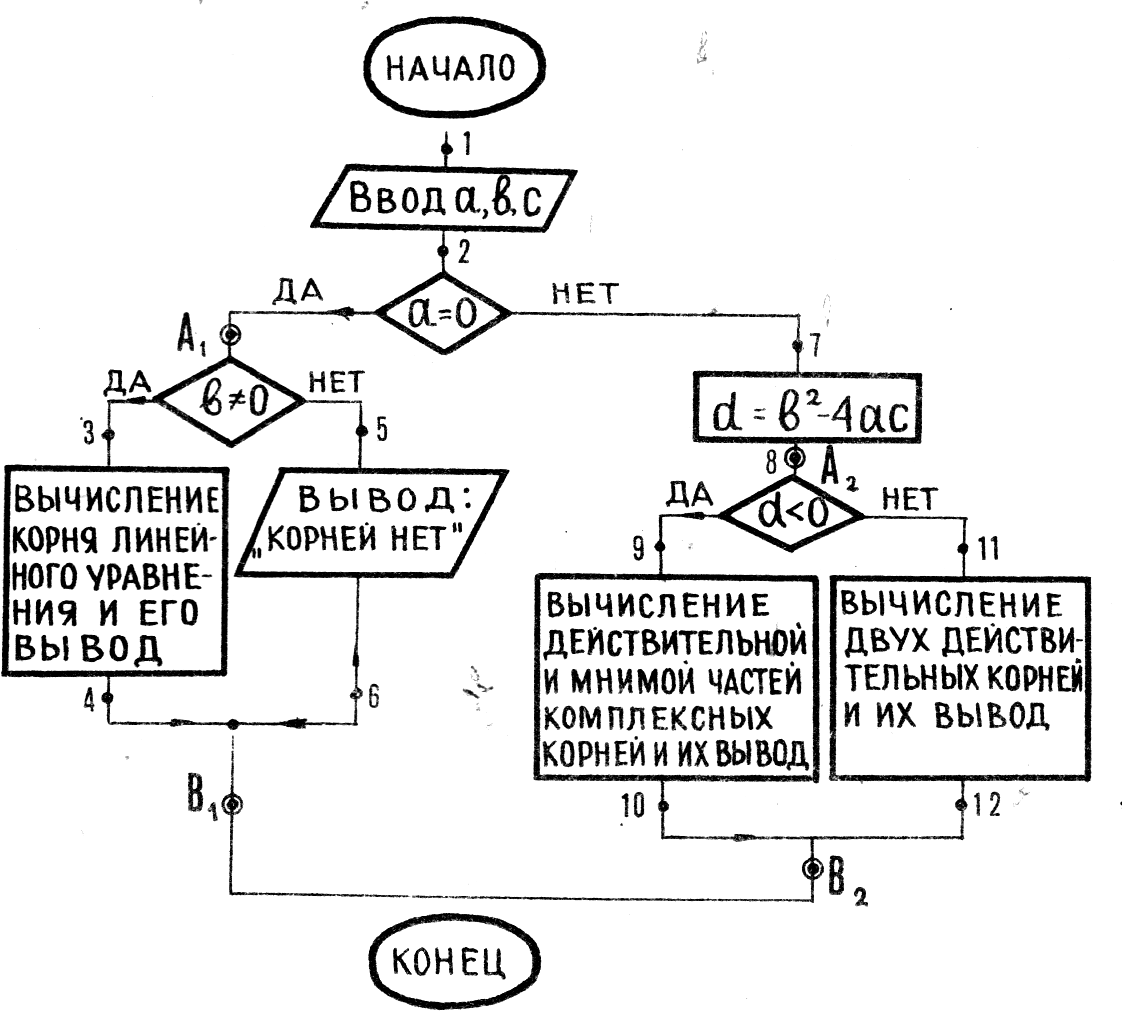
\includegraphics[width=0.5\textwidth]{sqroot_algo1}
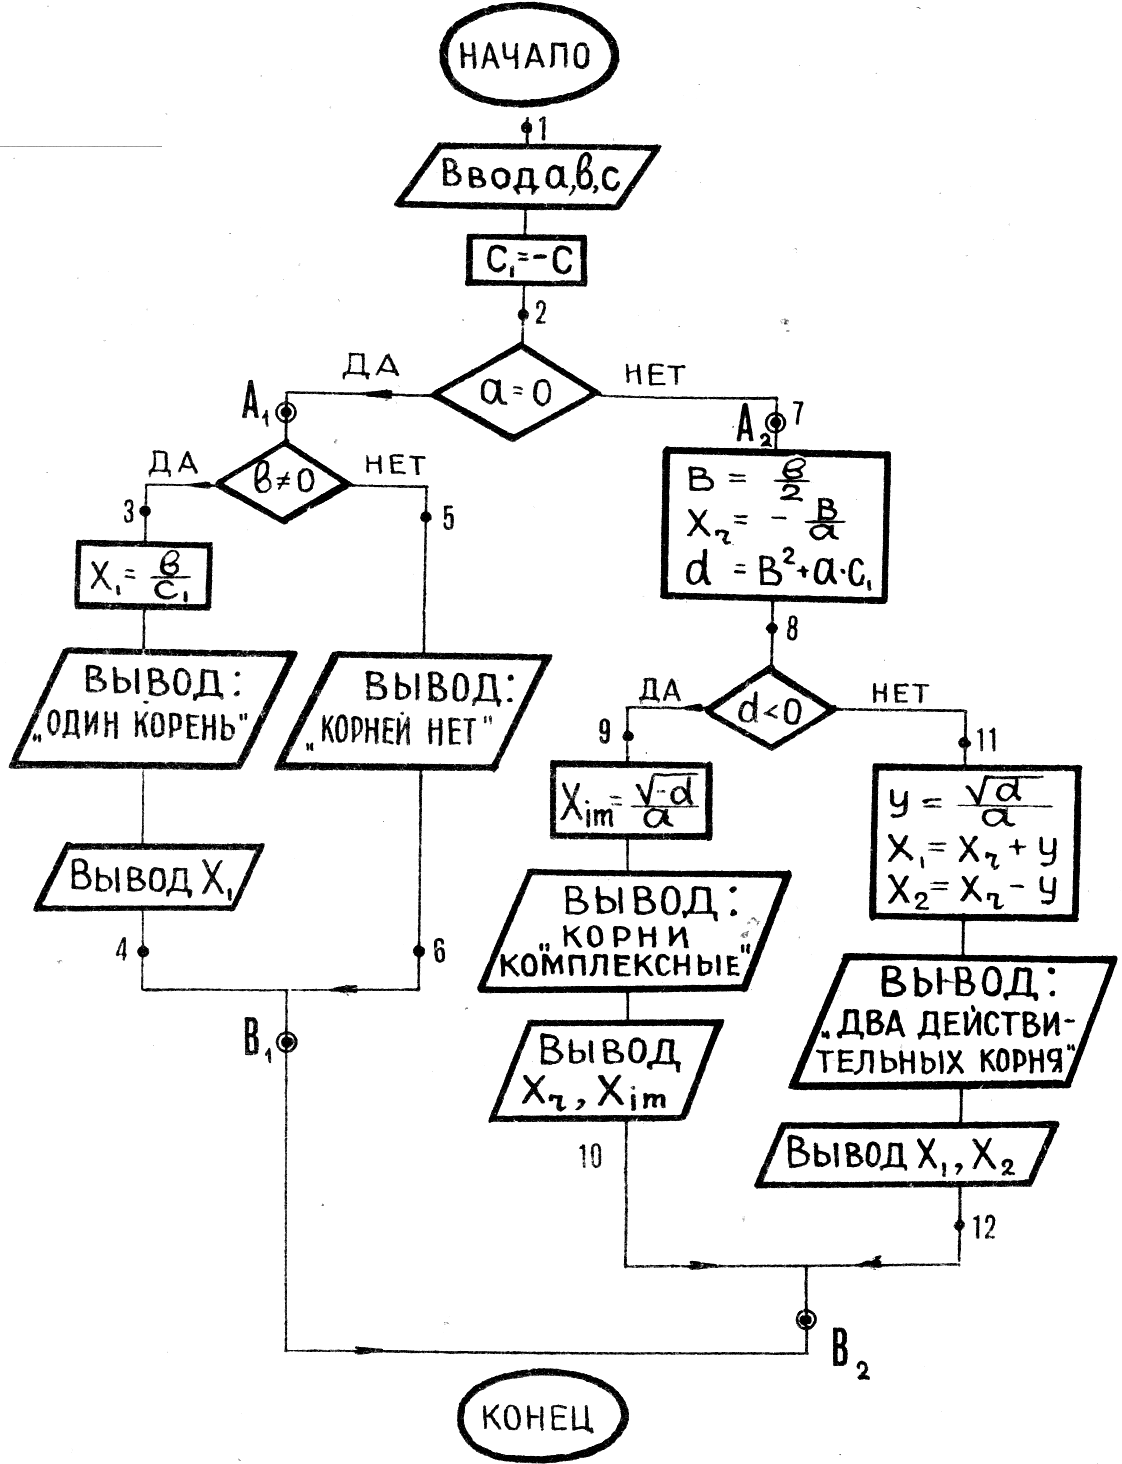
\includegraphics[width=0.5\textwidth]{sqroot_algo2}

Прежде чем приступить к написанию программы по блок-схеме, последнюю нужно детализировать, заменив словесные описания последовательностью формул. Чтобы различать отдельные части блок-схемы, мы пометили некоторые ее узлы цифрами. Детализация той ветви, что лежит между узлами 11 и 12, уже проведена: сюда надо просто вставить формулы из первого варианта блок-схемы. Для ветви 5-6 никаких формул не надо — вся работа на этом этапе заключается в выводе сообщения: «Корней нет». Остались две ветви. Для одной из них, 3-4, требуется всего одна формула:

\begin{equation}
x_{1}=-\frac{c}{b}
\end{equation}

А вот формулы для последней ветви 9-10:

\begin{equation}
B=\frac{b}{2}; d=\sqrt{B^{2}-ac};
\end{equation}
\begin{equation}
x_{r}=-\frac{B}{a}; x_{im}=\frac{d}{a}
\end{equation}

Здесь $x_{r}$ и $x_{im}$ — действительная и мнимая части комплексных корней, которые с помощью так называемой мнимой единицы, величины $i=\sqrt{-1}$, выражаются формулами:
$x_{1}=x_{r} + ix_{im}; x_{2} = x_{r} — ix_{im}$ Легко видеть, что в формулах для ветвей 9-10 и 11-12 много общего. Это означает, что одни и те же последовательности команд будут написаны дважды. Можно ли обойтись без такого дублирования? Да. Целесообразно выполнять общие для каких-то ветвей вычисления еще до разделения ветвей. Заметим также, что во всех формулах коэффициент с используется со знаком минус. Казалось бы, все равно, какую операцию использовать — сложение или вычитание. Но здесь надо учитывать специфику микрокалькулятора. Перед вычитанием пришлось бы правильно расставить по регистрам стека вычитаемое и уменьшаемое: первое — в X, второе - в Y. При сложении расстановка слагаемых значения не имеет, поэтому сложение предпочтительнее. Целесообразно заблаговременно сменить знак коэффициента, лучше всего сразу после его ввода. Все эти соображения учтены в новом варианте блок-схемы.

Вот теперь можно уже писать программу. Отметим, что наша блок- схема пригодится при составлении программы для любой ЭВМ и на любом языке программирования. Она подобна записи мелодии, которую затем можно аранжировать для любого инструмента с учетом его специфики...

Специфика микрокалькулятора проявляется, в частности, в двух моментах. Во-первых, у него разделены области памяти для хранения программ и данных. Во-вторых, ПМК оперирует только цифрами — буквенных символов в его языке нет. В силу первой особенности приходится вручную распределять информацию по регистрам, а вторая заставляет шифровать цифрами сообщения об особенностях решения (в нашем случае — о количестве и природе корней).

С распределением переменных по регистрам справляемся без труда. Предварительно намечаем такой вариант:

$a \rightarrow A; b \rightarrow B; c (c1 = -c) \rightarrow C;
x_{1} (x_{r}) \rightarrow 1(X); x_{2}(x_{im}) \rightarrow 2(Y)$.

Почему этот вариант предварительный? Да потому, что в процессе составления программы могут понадобиться дополнительные регистры или, наоборот, какие-либо из запланированных окажутся лишними.
Придумать систему шифров для необходимых сообщений тоже нетрудно. Скажем, появление на индикаторе нуля означает: «Корней нет», появление единицы — «Имеется один корень» и т. д. Часто так и поступают. Однако у этого метода есть существенный недостаток: можно спутать шифрованное сообщение с результатом вычислений. К счастью, есть и другой путь.

Мы уже знаем, что в микрокалькуляторе используются и такие символы для записи шестнадцатиричных чисел, которые не спутаешь ни с одной десятичной цифрой. Оказывается, есть возможность, формально выполняя некоторые «противозаконные» операции, получать на индикаторе и запоминать в адресуемых регистрах комбинации этих символов с обычными цифровыми. Их-то и удобно использовать в качестве сообщений; как их получать, скажем позже, а пока договоримся использовать следующие шифры: Е00	— «Корней нет», Е01 — «Один корень», Е02 — «Два действительных корня» и Г. — «Корни комплексные». Для хранения шифров тоже нужны регистры. Поэтому в дополнение к предварительному распределению памяти запишем: Е00→0, Е02→4, Е01→3, Г.→5. (Цифрами 0, 3, 4, 5, как и раньше, обозначены номера адресуемых регистров.)

Далее нужно продумать организацию ввода и вывода информации. Можно, конечно, вводить значения коэффициентов сразу в соответствующие адресуемые регистры в режиме вычислений, а результаты читать, вызывая на индикатор содержимое нужных регистров после останова, Однако большое число требуемых для этого ручных операций и необходимость постоянно помнить, что куда вводить и что откуда выводить, резко увеличат общее время получения результата, да и возможность ошибок возрастет. Лучше организовать ввод и вывод так, чтобы введенные числа автоматически рассылались по нужным регистрам и чтобы для прочтения результатов приходилось бы нажимать как можно меньше клавиш.

Остановимся на такой структуре ввода-вывода: коэффициенты вводятся в естественной последовательности — a, b, c; окончанием каждого ввода является нажатие клавиши С/П; после останова на индикаторе появляется шифрованное сообщение о характере результата, затем, после нажима С/П и следующего останова, высвечивается один корень, а после нажима клавиши ХУ — второй (если он есть),

Все технические требования к программе изложены, можно приступать непосредственно к ее составлению. Рекомендуем записывать программу так, как показано на рисунке, — указывать, кроме самих команд, их адресов и кодов, еще и содержимое регистров стека, хотя бы тех, которые могут понадобиться в дальнейшем. Желательно оставить еще одну колонку для кратких примечаний. Они помогут ориентироваться в программе — иной раз легче написать новую, чем разобраться в старой. Мы же в первом примере используем подробные примечания.

\begin{table}[H]
\begin{tabular}{|l|l|l|l|l|l|l|l|l|l|l|l|l|l|l|l|}
\rotatebox{90}{АДРЕС} & \rotatebox{90}{КОМАНДА} & \rotatebox{90}{код} & стек   &     &     &   &    & \rotatebox{90}{АДРЕС} & \rotatebox{90}{команда}& \rotatebox{90}{код} & стек    &     &    &   &        \\
      &         &     & X      & У   & z   & т & XI &       &     &     & X           & y   & Z  & т & X1     \\
00    & ПА      & 4-  & a      &     &     &   &    & 31    & ИПА & 6-  & а    & B   & d  &   &        \\
01    & с/п     & 50  & b      & а   &     &   &    & 32    & ÷   & 13  & B/a  & d   & а  &   &        \\
02    & ↑       & 0Е  & b      & b   & а   &   &    & 33    & /-/ & 0L  & $x_{r}$& d   & а  &   &        \\
03    & с/п     & 50  & c      & b   & а   &   &    & 34    & П1  & 41  & $x_{r}$& d   & а  &   &        \\
04    & /-/     & 0L  & $-c=c_{1}$& b  & а   &   &    & 35    & XY  & 14  & d    & $x_{r}$&    &   &        \\
05    & ИПА     & 6-  & а      &$ c_{1}$& b   &   &   & 36    & Fx\textless{}0 & 5C  &      &     &    &   &        \\
06    & Fx=0    & 5Е  &        &     &     &   &    & 37    & 48  & 48  &      &     &    &   &        \\
07    & 23      & 23  &        &     &     &   &    & 38    & /-/ & 0L  & -d   & $x_{r}$& а  &   &        \\
08    & FO      & 25  & $c_{1}$  & b   & а   &   &    & 39    & F√  & 21  & $\sqrt{-d}$  & $x_{r}$  & а  &   & \\
09    & XY      & 14  & b      & $c_{1}$&     &   &   & 40    & ИПА & 6-  & а    & $\sqrt{-d}$ & $x_{r}$ &   &        \\
10    & Fx≠o    & 57  &        &     &     &   &    & 41    & ÷   & 13  & $(\sqrt{-d})/a$ & $x_{r}$  &    &   & \\
11    & 19      & 19  &        &     &     &   &    & 42    & ИП5 & 65  & Г.   & $x_{im}$ & $x_{r}$ &   &        \\
12    & ÷       & 13  & $c_{1}/b$ &     &     &   &   & 43    & с/п & 50  &      &     &    &   &        \\
13    & ИП3     & 63  & Е01    & $x_{1}$&     &   &   & 44    & FO  & 25  & $x_{im}$  & $x_{r}$  &    &   &        \\
14    & с/п     & 50  &        &     &     &   &    & 45    & с/п & 50  &      &     &    &   &        \\
15    & XY      & 14  & $x_{1}$  & E01 &     &   &    & 46    & БП  & 51  &      &     &    &   &        \\
16    & с/п     & 50  &        &     &     &   &    & 47    & 59  & 59  &      &     &    &   &        \\
17    & БП      & 51  &        &     &     &   &    & 48    & F√  & 21  & $\sqrt{d}$   & $x_{r}$  & а  &   &        \\
18    & 59      & 59  &        &     &     &   &    & 49    & ИПА & 6-  & а    & $\sqrt{d}$  & $x_{r}$ &   &        \\
19    & ИП0     & 60  & Е00    & b   &     &   &    & 50    & ÷   & 13  & $(\sqrt{d})/a$  & $x_{r}$  &    &   &        \\
20    & с/п     & 50  &        &     &     &   &    & 51    & +   & 10  & $x_{r}+(\sqrt{d})/a$  &     &    &   &        \\
21    & БП      & 51  &        &     &     &   &    & 52    & ИП1 & 61  & $x_{r}$   & $x_{1}$  &    &   & $(\sqrt{d})/a$ \\
22    & 59      & 59  &        &     &     &   &    & 53    & FBx & 0   & $(\sqrt{d})/a$  & $x_{r}$  & $x_{1}$ &   &        \\
23    & X       & 12  & $ac_{1}$ & b   & а   &   &    & 54    & -   & 11  & $x_{r}-(\sqrt{d})/a$ &     &    &   &        \\
24    & XY      & 14  & b      & $ac_{1}$& а   &      & 55    & ИП4 & 64  & Е02  & $x_{2}$  & $x_{1}$ &   &        \\
25    & 2       & 02  & 2      & b   & $ac_{1}$& а &  & 56    & с/п & 50  &      &     &    &   &        \\
26    & ÷       & 13  & $b/2=B$  & $ac_{1}$ & а   &   & & 57    & FO  & 25  & $x_{2}$   & $x_{1}$  &    &   &        \\
27    & ПВ      & 4L  & B      & $ac_{1}$ & а   &   & & 58    & с/п & 50  &      &     &    &   &        \\
28    & $Fx^{2}$  & 22  & $B^{2}$  & $ac_{1}$ & а   &   & & 59    & БП  & 51  &      &     &    &   &        \\
29    & +       & 10  & $B^{2}+ac_{1}$ & а   &&  &    & 60    & 00  & 00  &      &     &    &   &        \\
30    & ИПВ     & 6L  & B      & d   & а   &   &    &       &     &     &      &     &    &   &       
\end{tabular}
\end{table}

«Ввод а». Эта операция выполняется перед пуском программы. Величина а набирается на клавиатуре. Набор заканчивается нажимом клавиши С/П.

00. Запись а в адресуемый регистр А.

01. Останов для ввода b. Набираем значение коэффициента на клавиатуре и снова нажимаем С/П.

02. Подготовка стека для приема значения с.

03. Введен третий параметр уравнения, коэффициент с. Ввод закончен. Теперь клавиша С/П запускает программу на счет.

04. Вычисляем $c_{1} =-c$. (Внимание: задавать с в экспоненциальном виде нельзя; в этом случае команда 04 изменит знак не мантиссы, а показателя.)

05. Проще всего вызвать а из «собственного» регистра А.

06-07. В стеке ничего не меняется. Мы лишь проверили, равно ли нулю содержимое регистра X. Если да, то есть если уравнение вырожденное, будем выполнять команду по адресу 08 (ветвь A1-В1. Если нет — перейдем к команде, записанной по адресу 23 (ветвь А2-В2).

08-09. Две команды использованы только для того, чтобы вернуть в регистр X значение b. Казалось бы, можно обойтись и одной — ИП В. Но нужно «помнить о будущем» — скоро придется делить c1 на b, а при таком распределении чисел в стеке, как теперь, для этого все подготовлено.

10-11. Если b = 0, то перейдем к команде по адресу 19 (на ветвь 5-6), иначе — по адресу 12.

12-18. Вычисления по ветви 3-4.

12. Вот где пригодилось допущенное «излишество» (команды 08 и 09). Теперь мы сэкономили вызов величины $c_{1}$ и перемену местами содержимого регистров X и У. Кроме того, чтобы вызвать величину $c_{1}$ из адресуемого регистра, ее надо было бы предварительно туда записать. Мы же обходимся пока без записи величины $c_{1}$. Она к нашим услугам прямо в стеке.

13-14. Вычисления по ветви 3-4 закончены. Вызываем в регистр X сообщение Е01 из регистра 3, останавливаем программу, чтобы его можно было прочесть. Иначе говоря, реализуем блок «Вывод «Один корень».

15-16. После нажатия клавиши С/П отрабатываем «Вывод X1». Величина корня — на индикаторе.

17-18. Эта команда замыкает ветвь 3-4, управление передается последней команде программы (блоку «Конец»), все остальные ветви обходятся, и работа программы заканчивается.

19-22. Сюда мы попадаем только в том случае, если а=0 и b=0. Вычислений проводить не надо. Просто выводим на экран сообщение Е00, что означает «Корней нет», и замыкаем ветвь, подобно предыдущей.

23-34. Ветвь 7-8.

23. 	Если мы уж попали на эту команду, значит, уравнение невырожденное. Надо вычислять дискриминант, а потом корни по одной из двух ветвей. Кстати, вас не смущает, что командой 12 мы вроде бы распрощались с величиной $c_{1}$? Ведь она в адресуемый регистр так и не записана... Но не волнуйтесь, все в порядке. Если мы и попадаем на адрес 23, то обязательно сразу после команды по адресу 07, а все промежуточные команды не выполняются. Поэтому и содержимое стека такое же, как и до команды перехода. Все готово для умножения $ac_{1}$ Вот после этой команды величина $c_{1}$ потеряна для нас навсегда. Но она больше и не нужна.,

24. 	Выдвигаем величину b на первый план. Она теперь — объект работы нескольких команд.

25-27. Вводим в регистр X число 2, делим на него b и запоминаем результат в регистре В,

28-29.	Величина В возведена в квадрат, дискриминант вычислен. Однако прежде чем перейти к его анализу,	нужно получить величину $x_{r}$, так как она понадобится нам в обеих ветвях.

30. 	Извлекаем величину В из ее хранилища — регистра В.

31. 	Для деления нужна величина а. Проще всего вызвать ее в стек заново.

32-34. Теперь все вычисления по ветви 7-8 закончены. Величина $x_{r}$ отправлена на хранение в регистр 1, можно переходить к анализу величины d, благо она рядом.

35-37. Делаем последнее сравнение в программе. Если d>0, то корни действительные и надо перейти на ветвь 11-12 (команда 48). Если же d<0, то корни комплексные, надо вычислять их по формулам ветви 9-10.

38-47. Ветвь 9-10.

38-39. Так как величина d меньше нуля, то, чтобы вычислить корни, нужно сначала изменить ее знак.

40. 	Для вычисления $x_{im}$ нужна величина а. Проще всего опять-таки вызвать ее из регистра А.

41. 	Величина $x_{im} = \sqrt{(-d/a)}$ вычислена и находится в регистре X.

42-43. Все готово для вывода результата. Можно останавливать ПМК и считывать $x_{im}$ и $x_{r}$ с индикатора, но мы еще не вывели на индикатор сообщения о том, что за величины получены. Приходится отодвигать готовые результаты и переносить в регистр X шифрованное сообщение: Г. — «Корни комплексные».

44-45. Сообщение прочитано. Возвращаем результаты вычислений на старое место и останавливаем программу, чтобы считать их.

46-47. Ветвь 9-10 замкнута.

48-60. Последняя ветвь 11-12.

48. Поскольку d находится в регистре X (как и после команды 35), то сразу же извлекаем квадратный корень.

49-50. Вычисляем вспомогательную величину $\sqrt{d/a}$

51. 	Получаем первый корень $x_{1}$ Величина $\sqrt{d/a}$ перешла в регистр
предыдущего результата X1.

52-54. Вычисляем второй корень $x_{2}$. Расчеты закончены.

55-58. Вывод результатов организуется так же, как и в предыдущей ветви.

59-60. Вот и последние команды, реализация блока «Конец». Они подготавливают программу для приема новой информации, передавая управление на начало. Можно вводить новые данные и повторять расчет.

Вернемся к распределению памяти. Окончательная картина такова:

а→А; b→В; $x_{r}$→1;
$x_{r}$, $x_{1}$→Y; $x_{im}$, $x_{2}$→X,

Итак, три регистра удалось сэкономить. Если бы нам понадобилось ввести в оставшуюся часть программной памяти еще одну программу, то «лишние» регистры очень бы пригодились.

Теперь, как и было обещано, о получении шифрограмм. Сообщение Е00 получается, если в режиме вычислений выполнить следующие действия. Сначала набрать 100 ВП 99. На индикаторе, естественно, загорается ЕГГОГ. Не смущаясь, продолжаем: ВП ↑. На индикаторе то, что надо: Е00. Нажимаем ПО — и шифрограмма отправляется на хранение в регистр 0.

Е01 и Е02 получаются аналогично, только вместо числа 100 нужно набрать соответственно 101 или 102. Алгоритм же для получения сообщения Г. другой: Сх ↑ ÷ (здесь, конечно, опять ЕГГОГ, ведь делится ноль на ноль), ВП ВП ↑. На индикаторе — то, что нужно. Можно теперь записать Г. в регистр 5.

Программа закончена. Не слишком ли она велика? Ведь уравнение, казалось бы, элементарное... Но фактически написаны четыре разные программы, каждая из которых рассматривает отдельный вариант уравнения, плюс еще одна, которая выбирает нужную из этой четверки. Это не так уж мало. Впрочем, программу можно действительно сократить. Как это делать, мы еще расскажем.

С другой стороны, работа еще не закончена. Специфика ПМК проявляется в том, что решение любой задачи на нем автоматизировано не полностью, оно реализуется совместными усилиями человека и микрокалькулятора. Программу для ПМК мы написали, а вот инструкцию, «программу для человека», пока еще нет. Такая инструкция необходима. Вот как она может выглядеть.

\begin{enumerate}
\item Ввести программу.
\item Установить режим вычислений (F АВТ).
\item Ввести шифры:

100 	ВП 99 ВП ↑ ПО

101 	ВП 99 ВП ↑ ПЗ

102 	ВП 99 ВП ↑ П4 

Сх ↑÷ ВП ВП ↑ П 5

\item Очистить программный указатель (В/О).
\item Ввести исходные данные: а С/П; b С/П; с С/П.
\item Вывод: после первого останова на индикаторе появляется сообщение:

Е00 — корней нет;

Е01 — уравнение линейное, корень только один;

Е02 — два действительных корня; 

Г, — корни комплексные.

\item Если корней нет, то для продолжения расчетов перейти к п. 5. Если корни есть, то нажать С/П. После останова на индикаторе — значение первого корня (если корни действительные) или мнимой части комплексных. Для чтения другого корня или действительной части нажать ХУ
\item Для продолжения расчетов перейти к п. 5.
\end{enumerate}

\textbf{Контрольный пример:}

Ввод:

а =2; b = 5; с=3

а=1; b=-4; c=5 

а=0; b = 8; с=3 

а = 0; b = 0; c=1

Вывод: 

Е02; -1; -1,5 

Г; 1;	2

Е01; $-3,75*10^{-1}$ 

Е00

\section{Истинная правда}
МИХАИЛ ПУХОВ

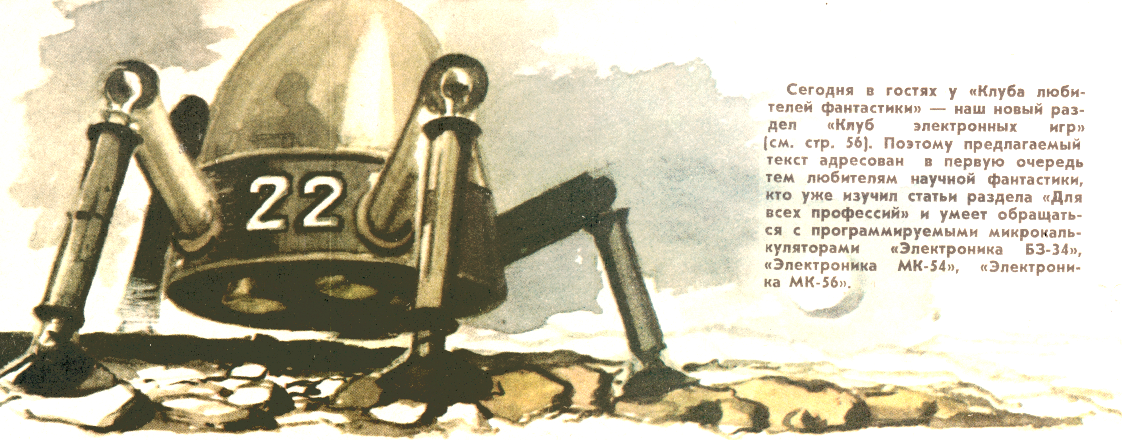
\includegraphics[width=0.5\textwidth]{real_truth}

"Громадный метеорит врезался с космической скоростью в наш звездолет и пробил его насквозь, оставив в обшивке дыру размером с человеческую голову. Воздух со свистом хлынул наружу".

«Пилот наконец решился и нажатием кнопки отправил в реактор последние остатки топлива. На космонавтов обрушилась десятикратная перегрузка. Тысячетонная громадина корабля дрогнула и медленно двинулась вверх. Люди были спасены».

Подобными эпизодами изобилуют поступающие в редакцию «ТМ» рассказы начинающих фантастов. Рецензировать такие произведения затруднительно. Интуитивно ясно, конечно, что после столкновения с «громадным метеоритом" от звездолета ничего не останется, а «последних остатков топлива» не хватит, чтобы даже при «десятикратной перегрузке» обеспечить взлет «тысячетонной громадины корабля» со сколько-нибудь приличной планеты. Но какими аргументами подкрепить интуитивные соображения? Не будешь же каждый раз проделывать громоздкие вычисления по соответствующим формулам — рассказов в отдел фантастики приходит ежедневно около десяти. Где взять время для этих проверок?

К счастью, в нынешнем году на страницах журнала открылась новая рубрика «Для всех профессий», и в редакции появился программируемый микрокалькулятор «Электроника МК-54». Поскольку ошибки наших авторов легко подразделить на несколько четко выраженных классов, я составил десяток программ для ПМК, в которые заложены наиболее типичные фантастические ситуации. Вводя в машинку различные соображения относительно размеров «громадного метеорита» и величины его «космической скорости», через минуту я получаю число, на основании которого со спокойной совестью отвечаю: «К сожалению, при самых оптимистических предположениях насчет размеров и скорости придуманного Вами метеорита диаметр проделанной им дыры в обшивке значительно превысил бы длину звездолета, то есть последний попросту превратился бы в пар, так что увлекательные приключения Ваших героев после такого столкновения никоим образом не могли иметь места. Рукопись возвращаем..."

Есть среди моих проверочных программ и такая, которая рассчитывает взлет с безатмосферных планет и посадку на их поверхность. Тот, кто внимательно изучил материалы рубрики «Для всех профессий», разберется в ней без труда. Вот эта программа:

00. ИПД 01. Fx<0 02. 09 03. ↑ 04. ИП8 05. ÷ 06. XY 07. ПП 08. 90 09. ИПА 10. Fx≠0 11. 43 12. Fx<0 13. 33 14. 2 15. X 16. ↑ 17. ИП4 18. ИП3
19. 	— 20. X 21. ИПВ 22. $Fx^{2}$ 23. + 24. F√ 25. ИПВ 26. — 27. ÷ 28. ↑ 29. ИП8 30. X 31. БП 32. 90
33. 	ИПД 34. Fx≠0 35. 86 36. ИП3 37. $Fx^{2}$ 38. F√ 39. ИП7 40. — 41. Fx<0 42. 87 43. ИПВ 44. ИПА
45. С/П 46. П1 47. П2 48. Fx≠0 49. 43 50. ÷ 51. П8
52. 	ИП5	53.	ИПД 54. + 55. ÷ 56. ИП6 57. X 58. П3
59. ИП4	60.	— 61. ИП2 62. X 63. ИПВ	64.	+ 65. ПВ
66. FBx 67. + 68. 2 69. ÷ 70. ИП2 71. X 72. ИПА
73. 	+ 74. ПА 75. ИПС 76. ИП2 77. ИПО 78. X 79. — 80. ПС 81. ИПД 82. ИП1 83. — 84. ПД, 85. В/О
86. ИП6	87.	ИП9 88. С/П 89. Сх 90. П1 91. XY 92. П2
93. 	Fx<0 94. 50 95. ИПЗ 96. БП 97. 59

Подробная инструкция к этой программе (условно она называется «Лунолет-1») и описание увлекательной компьютерной игры, в которую можно играть с ее помощью, приведены на стр. 56. Но вернемся к проверке поступающих в редакцию материалов.

Надо сказать, что, помимо многочисленных писем, к нам довольно часто приходят посетители. Как правило, это весьма необычные люди. Один несет новый проект или действующую модель вечного двигателя либо безопорного движителя; другой рассказывает о встречах со «снежным человеком» и чудом дотянувшими до наших дней мезозойскими динозаврами. А года два назад в редакции появился человек, который категорически утверждал, что он якобы... провалился к нам из будущего, из конца XXI века!

Этот человек бывал у нас на протяжении двух недель. И каждый раз рассказывал что-нибудь о будущем. Мы внимательно все выслушивали (так полагается по долгу службы), записывали его рассказы на магнитофон. Ничего, впрочем, особенного в них не было — любой из нас при желании мог придумать и не такое. Да и как проверить? Потом он куда-то пропал, и вскоре все забыли о нем.

А недавно возникла мысль: теперь, когда у меня есть мои проверочные программы, я могу с помощью ПМК проанализировать и рассказы этого человека. Ведь все записано на пленку, а пленки хранятся в архиве!

Какое-то время ушло на розыски и подготовительную работу. И вот передо мной расшифровка старой магнитофонной записи. Рядом — готовая к вычислениям «Электроника».

Приготовьтесь и вы. Введите в свой ПМК программу «Лунолет-1» и переведите машинку в режим вычислений. Будем работать вместе.

Вот одна из его историй. (В скобках — наши краткие комментарии.)

Я управлял космическим кораблем один-единственный раз в жизни.

Конечно, в юности, как и многие мои сверстники, я мечтал стать космонавтом. Но мечты эти развеялись на первой же медкомиссии: при перегрузках больше трех «же» мне становилось плохо. А тех, кто не выдерживал пятикратной, к дальнейшим испытаниям не допускали. Волей-неволей пришлось забирать документы. Я подал на вычислительную технику, через шесть лет благополучно защитил диплом и — ирония судьбы! — был направлен по распределению на Луну, в Центр имени С. П. Королева. Там я работаю до настоящего времени.

После того как по соседству нашли неорганическую нефть, Центр сильно разросся. Теперь это настоящий город с населением порядка трех тысяч человек. Прикрывающие его купола соединены туннелями. Как в метро, только стены прозрачные. Это, грубо говоря, большие трубы, протянутые прямо по лунной поверхности. Один из туннелей ведет к астровокзалу. Космопорт Центра — обширный комплекс, он обслуживает всю Солнечную систему. По роду работы я часто бываю в порту, потому что корабли напичканы электроникой, рано или поздно что-нибудь выходит из строя, а чинить вычислительную технику — это моя специальность и прямая обязанность.

Случай, о котором я упомянул, произошел летом 2087 года. Работа у нас строится циклически: четыре месяца трудимся, два отдыхаем. Как правило, на Земле. Родные тоже прилетают иногда погостить — пассажирская линия Земля — Луна открылась давно. В то лето ко мне прилетел сын, Сергей. Я не видел его несколько месяцев, за это время он сильно подрос. Ему скоро двенадцать, и он бредит космонавтикой. Мы с женой надеялись, что самостоятельное путешествие на Луну очень его обрадует. Да и сам он, как она сообщила, в ночь накануне вылета совсем не спал.

Но когда я встретил его на астровокзале, он выглядел разочарованным.

— Ерунда! — сказал он. — Сидишь в кресле, стюардесса носит конфеты и воду в тюбиках. Как в самолете. Никаких перегрузок. Хоть и невесомость, но плавать по воздуху запрещают. Заставляют сидеть в кресле да еще и пристегиваться. Вот если бы самому в рубке сидеть за штурвалом и нажимать рычаги...

Он горько вздохнул и грустил минут пять, пока мы добирались домой. Потом отправился погулять. Вернулся через полчаса, разочарованный еще больше: на поверхность не выпускают, скафандр не дают, все кругом самое обычное, деревья и люди как на Земле. Никакой Луны нет. Разве что тяжесть поменьше, но это ему неинтересно — после двух-то суток невесомости на борту лайнера. Было уже поздно, и я уложил его спать, А потом и сам лег — завтра с утра на работу. Я пообещал взять его с собой: там интересно — вычислительные машины, манипуляторы и прочее.

Но наутро мне позвонили — появилось срочное дело. Я все записал, потом сварил кофе. Сергей был уже на ногах. Когда мы позавтракали, я сообщил, что планы изменились, так что пусть пока посидит дома. Он сначала возмутился, но потом смирился с необходимостью. Я пояснил, что буду в отсутствии каких- нибудь полтора часа.

— Папа! — сказал он. — А куда ты пойдешь?

— На космодром.

— A, — он разочарованно махнул рукой. — Я там уже был. Там скучно. Никуда не пускают.

— Мне не в порт, — объяснил я. — Мне на местные линии. Это небольшая площадка в стороне от главного поля. Лайнеров, на каком ты летал, там нет. Только лунолеты местного сообщения.

— Настоящие? — заинтересовался он.

— Разумеется, не игрушечные. Но они маленькие — всего две тонны сухого веса. Вернее, сухой массы. Здесь ведь все весит в шесть раз меньше, чем на Земле.

— Знаю, — отмахнулся Сергей. — А что ты там будешь делать?

— Работать, — пожал я плечами. — На одной из этих машин отказал киберпилот. Надо посмотреть. Если какой-нибудь пустяк, сделаю на месте. А если что-то серьезное...

— Ты пойдешь в рубку? — Глаза у него расширились.

Я невольно расхохотался.

— Какая там рубка! Кабина, два кресла. Не повернешься.

— Но приборы там? — продолжал он допрос. — Рычаги управления там?

— Конечно, — простодушно признался я. — Где же им быть еще?

— Возьми меня с собой, — потребовал он.

— Но это не игра, — попробовал я объяснить. — Это работа...

— Папа! — сказал он. — Ты мне обещал.

— Только не говори маме, — попросил я, сдаваясь.

Несколько минут спустя электрокар мчал нас по направлению к космопорту. Улицы в этот час были пустынны — все на работе. Незадолго до астровокзала мы свернули в боковой туннельчик, ведущий к служебному выходу. Сергей был в приподнятом настроении, что-то напевал.

На проходной я показал удостоверение вахтенному.

— А это что за гражданин?

— Он со мной, — сказал я. — Это мой сын.

— А где его документ? — спросил вахтенный.

— Ему не положено. Он еще маленький.

Минуту вахтенный размышлял. Ситуация, очевидно, была для него новой.

— Ладно, пускай идет. Под личную ответственность.

Скафандры нам выдали без проблем. Сережке, конечно, он был великоват, но только чуть-чуть —не такой уж он у меня маленький.

— Баллоны стандартные, — предупредил выпускающий. — На два часа. Справитесь?

— Конечно. Мне и часа хватит с гарантией. Двадцать минут туда, двадцать обратно, десять на месте. Ну и десять на всякие осложнения.

— Ясно, — добродушно сказал выпускающий. — Только пусть лучше осложнений не будет. Хорошо?

Я опустил забрало, и мы прошли в воздушный шлюз. А спустя короткое время уже шагали под голубым светом Земли. Была середина лунной ночи — на Земле в эти дни новолуние.

Сказать, что Сергей был восхищен, — значит, ничего не сказать. Он был ошеломлен. Похоже, он никак не ожидал, что ему выдадут скафандр. Настоящий, с индивидуальной системой жизнеобеспечения. На Земле я бы в таком весил килограммов сто пятьдесят, да и Сергей потянул бы на добрую сотню. Мы осторожно шагали по ровному реголиту — искусственного покрытия здесь никто не прокладывал, убрали крупные камни, и все. Не для важных персон. Но дорожка была ухоженной. До нас здесь ходили многие — все, кто работал на дальних лунных базах и опорных пунктах. Строители, ученые, инженеры...

— А там что такое? — Сергей вновь обрел способность задавать вопросы. Его голос в моем шлемофоне звучал непривычно.

Он показывал направо. Там выступали из-за горизонта массивные строения промышленного блока.

— Это тебе неинтересно, Сережа, — сказал я. — Там качают нефть и гонят из нее керосин. Для двигателей. — Я махнул в сторону космопорта. — И еще вырабатывают жидкий кислород.

— Для скафандров? — Он произнес слово «скафандр» с особенным выражением. Я усмехнулся:

— И для скафандров, конечно. Но в основном его везут на те же заправочные станции. Горючее ведь не будет гореть без окислителя.

Некоторое время мы шагали в молчании. Идти стало чуть труднее — дорожка поднималась к вершине обычного для Луны плоского холма. Еще сотня шагов — и мы достигли места своего назначения. Нашим глазам открылась стоянка лунолетов.

Их было десятка два — старые, но надежные машины. В первом приближении это скругленный конус высотой метра три с половиной, опирающийся на четыре амортизатора типа «паучья нога». Вся верхняя часть прозрачна, для облегчения обзора. Это и есть та самая «рубка», в которую так рвался мой сын.

На боку каждого лунолета стоял опознавательный номер — две цифры, начертанные светящейся краской и обведенные черной каймой. Наш был с краю. Без дополнительных приключений мы забрались внутрь. При виде многочисленных циферблатов у Сергея разгорелись глаза.

— Это настоящий корабль? — спросил он.

Я понял. На Земле похожие машины стоят в каждом парке отдыха. Аттракционы. Влезай в люк и испытывай всякие ощущения.

— Самый что ни на есть, — сказал я.

— А как им управлять?

Я усмехнулся.

— Проще простого. Вот этот ящик, — я указал пальцем, — называется киберпилот. Если тебе нужно попасть, допустим, на базу «Циолковский», ты набираешь на пульте задание, потом нажимаешь вот эту кнопку, и киберпилот благополучно доставляет тебя куда надо. Но сейчас именно он-то и неисправен.

Это Сергея на время утихомирило. Он, видимо, ожидал чего-нибудь в духе земных аттракционов, когда сам даешь вводные и тебя швыряет в разные стороны. Я аккуратно снял с киберпилота пломбу и сдвинул лицевую панель. На вид все в порядке. Дал на схему напряжение. Циферблаты на пульте ожили.

Где же искать повреждение?..

— А это что за рычаги? — услышал я голос Сергея.

Я обернулся. Оказывается, он устроился во втором кресле. Играл в космонавта. Указывал он на рычаги ручного управления двигателем.

— Это для посадки, — объяснил я. — Киберпилот всегда доставит тебя куда надо, но он не знает местность. Вдруг там трещина, скажем, или какой-нибудь камень. Тогда нужно дать небольшой импульс, чуть притормозить спуск, чтобы машина проскочила опасное место.

Я опять повернулся к киберпилоту. Однако не тут-то было.

— А как дать импульс? — спросил Сергей.

— Ты мне мешаешь, — сказал я. — Откуда мне знать? Впрочем, гляди: написано «Расход топлива» и цифры, ага, в килограммах. Рычаг стоит здесь, значит, ты собираешься истратить 65 килограммов топлива. А возле правого рычага — «Время» и тоже цифры. Это, видимо, время, за которое ты собираешься свое топливо израсходовать. Меньше время — больше тяга, а если время больше — тяга соответственно меньше. Сейчас рычаг стоит на цифре три. Значит, если ты подашь эту команду на двигатель, он израсходует 65 килограммов за три секунды.

— А это много?

— Не знаю, — сказал я. — По-моему, все равно что ничего.

— А как подать команду на двигатель?

— Откуда я знаю? — огрызнулся я. — Ты мне мешаешь. Пульт наверняка заблокирован, а баки пусты. Полюбуйся, — я ткнул пальцем в индикатор, — Видишь? «Топливо», четыреста. Всего-навсего! А шкала на две с половиной тонны.

— А как... — продолжал он допрос.

— Отстань от меня! — скомандовал я. — Ты мне мешаешь. Скажешь еще хоть слово, тут же идем домой. И вообще, отошлю тебя к маме.

Он обиженно умолк, а я занялся киберпилотом. Набрал контрольный тест — он прошел нормально. Набрал второй — тоже полный порядок. Что они там, спятили? Совершенно исправная машина. Я набрал третий тест. И тут началось...

\textbf{
(Пока рассказчик работает с вычислительной техникой, поработаем немного и мы. Не будем забывать о своей главной задаче — вывести его на чистую воду. Кульминационный момент, судя по всему, приближается, самое время нажимать клавиши ПМК. Программа введена, формируем и отправляем в регистр 9 аварийный сигнал Г: Сх ÷ ВП ВП ↑ П9. Теперь исходные данные. Дело происходит на Луне, ускорение свободного падения 1,62 м/c$^{2}$. Набираем на клавиатуре 1,62 П4. Масса корабля без горючего две тонны, сюда нужно добавить массу рассказчика вместе со скафандром (150 кг) и его сына (100 кг). Набираем 2250 П5. Двигатель, очевидно, работает на керосине и жидком кислороде, скорость истечения 3660 м/с. Набираем это число на клавиатуре и нажимаем П6. Очередь за предельным ускорением. По словам рассказчика, ему становится плохо уже при трех «же». Набираем на клавиатуре 9,81 ↑ 3 X П7. Скорость и высота равны нулю — нажимаем 0 ПА ПВ. Запас топлива 400 кг. 400 ПД. Вводим в регистр С ресурс жизнеобеспечения в секундах. Воздуха в баллонах было на два часа, двадцать минут герои повествования шли до стоянки, возятся минут двадцать, да надо еще накинуть двадцать на обратный путь. «На всякие осложнения» им остается ровно час. Набираем 3600 ПС и соответственно I ПО. Исходные данные введены. Нажимаем В/О и С/П. Через секунду на экране загорается высота — ноль. Нажимаем XY. На экране скорость — тоже ноль. Все правильно. Можно во всеоружии ждать грядущих событий. А они, несомненно, вот-вот последуют.)
}

...Ни один контрольный тест не проходил. Я бросил взгляд на часы: с момента, когда мы покинули воздушный шлюз, прошло уже сорок минут. Пора возвращаться. Я потянулся к рубильнику — снять с оборудования напряжение — и посмотрел на сына. Он продолжал играть в космонавта: нажимал какие-то кнопки,. созерцал пляшущие на экранах кривые. Рычаги управления тягой стояли в прежнем положении. Он положил указательный палец на большую красную клавишу. Неясное предчувствие шевельнулось у меня в голове.

— Не смей! — крикнул я.

Но было поздно. Под нами загрохотало, за прозрачным колпаком взметнулось пламя, чудовищной силы удар швырнул меня в кресло, и у меня потемнело в глазах...

\textbf{
(Значит, пульт все-таки заблокирован не был и команда прошла на двигатель. Не особенно, конечно, убедительно, но нас интересует фактическая сторона дела. Двухтонная машина, жалкие 60 кг топлива, и вдруг — «чудовищной силы удар»! К счастью, проверить данный эпизод нетрудно. Подадим ту же команду и на свой пульт: 65 ПП 3 С/П. На экране мелькают цифры, потом... загорается аварийный сигнал Г! Как это ни удивительно, перегрузка действительно превысила допустимую, рассказчик потерял сознание и какое-то время после отсечки двигателя не сможет управлять лунолетом. Снова нажимаем С/П.)
}

...Когда я очнулся, кругом было только небо. Сколько я был без сознания? Не знаю. Но мы падали, падали со страшной скоростью! Очевидно, за время моего беспамятства ракета прошла вершину траектории и теперь стремительно неслась вниз. Сергей тянулся к рычагам управления. Но игры кончились. Какую-то секунду я не мог опомниться, но еще через секунду был у пульта. Что я мог успеть в такой ситуации? Заметил лишь показания индикаторов — скорость восемьдесят, высота триста с чем-то.

— Папа! - крикнул Сергей.

Что я мог успеть? Не меняя режима двигателя, я ударил по красной клавише. На нас снова обрушилась перегрузка...

\textbf{
(На нашем же индикаторе высота полета 169 м — везде округляем до целых. Нажимаем XY. Скорость 84 м/с. Ну что ж, будем считать, проверка закончена. Скорость еще более-менее, но высота в рассказе завышена вдвое. Можно откладывать ПМК в сторону... Впрочем, пока он добирался до пульта, прошло еще две секунды. Две секунды свободного падения с выключенным двигателем. Но куда можно упасть за две секунды? Разве что на Луну — не в небо же! Ладно, для очистки совести засылаем соответствующую команду: 0 ПП 2 С/П. На экране зажигаются высота 334, скорость 81. Невероятно, но цифры совпали! Почему же он утверждает, что лунолет падал? Непонятно. Но набираем новую команду: 65 ПП 3 С/П. Опять сигнал Г — запредельные перегрузки! — вновь нажимаем С/П и ждем результата.)}

...Когда я очнулся снова, мы опять падали. Я рванулся к красной клавише, но взгляд мой упал на индикатор высоты. Почти километр! И цифры росли! Значит, мы вовсе не падали — мы неслись вверх со скоростью реактивного истребителя! И в прошлый раз мы, конечно же, тоже поднимались! Меня ввела в заблуждение невесомость. Мы действительно падали, но падали вверх! И я, болван, включив двигатель, только усугубил наше и без того тяжелое положение. Зато теперь появилось время, чтобы собраться с мыслями...

\textbf{
(Не так-то просто, оказывается, поймать его на слове! У нас очередной останов. Высота 916 м — действительно, почти километр, —- скорость 166 м/с. Примерно 600 км/ч. Маловато, конечно, для истребителя, но... Можно ли считать это серьезной ошибкой? Будем объективны, оставим рассказчику право на художественное преувеличение. Как бы то ни было, включать двигатель он вроде цока не собирается, так что нашему ПМК можно тоже дать передышку.)}

...— Папа! — сказал Сергей, выбираясь из-под меня. — А почему ты говорил, что 65 килограммов — это все равно что ничего?

— Отстань от меня! — приказал я, — Марш во второе кресло и пристегнись!

Я проследил, как он это выполнил, и пристегнулся сам. Цифры на индикаторе высоты увеличивались, но все медленнее и медленнее. На киберпилот надежды нет, придется выкручиваться самому. Но пока, пожалуй, лучше не делать ничего. Гнать вверх бессмысленно. Вниз (а рядом с красной клавишей я углядел другую, «Реверс тяги») — еще хуже. Вот начнем падать, тогда... Я заранее установил рычаги в положение 25 кг и 2 с и ждал. Да, я сильно ошибся насчет этих килограммов. Похоже, в них большая сила...

— Папа! — подал голос Сергей. — А мы сможем улететь в космос?

— Отстань! — рявкнул было я, но вдруг у меня защемило сердце. Ребенок не понимал, что мы на волосок от гибели, для него это было игрой! — Сереженька, — сказал я как можно ласковее, — в космос мы с тобой еще слетаем. Но сейчас, пожалуйста, помолчи...

Мы взлетели уже почти на десять километров. Цифры на указателе скорости дошли до нуля и начали медленно расти, теперь уже с отрицательным знаком. Когда скорость достигла примерно тридцати метров в секунду, я нажал красную клавишу. Высота к этому времени уменьшилась почти до девяти километров. Свободный полет продолжался ровно две минуты...

\textbf{
(Наконец-то появилась новая цифра, которую можно проверить. Две минуты с нулевой тягой. Команда: 0 ПП 120 С/П. После останова высота 9175, скорость — минус 28. Опять все сходится! Новая команда: 25 ПП 2 С/П. Машинка рассчитывает маневр.)}

...На сей раз перегрузка была терпимой. На индикаторах мелькали цифры. Высота почти не изменилась, но мы опять поднимались! Что ж, мы так и будем болтаться на этой высоте, пока не кончится все топливо? И весь кислород?! В отчаянии я установил рычаги в положение 10 и 10 и дал реверс тяги. Лунолет кувыркнулся двигателем вверх. Далеко внизу я увидел постройки Центра, обширные поля космодрома и крошечное пятнышко площадки, с которой мы так неосмотрительно стартовали...

\textbf{
(У нас после останова высота 9151, скорость — чуть меньше пяти метров в секунду и, действительно, снова направлена вверх. Вводим команду 10 ПП 10 ПП /—/ С/П. После останова высота равна 9044 м, скорость — 26 м/с со знаком минус. Снова падаем, и довольно быстро.)}

...Скорость падения увеличивалась быстрее, чем я рассчитывал. Я решил притормозить: убрал реверс, установил 25 кг и 5 с и надавил на красную клавишу. Но она не поддалась. Видимо, эти пульты устроены так, что новая команда блокируется, пока не исполнена прежняя. И лишь когда десять секунд истекли, корабль вновь крутанулся двигателем вниз. Но когда тот выключился, мы оставались все на тех же девяти километрах и опять, хоть и очень медленно, поднимались!..

\textbf{
(Команда: 25 ПП 5 С/П. Результат: высота 8984, скорость два с половиной метра в секунду, снова со знаком плюс. Он что, действительно собирается провести здесь всю оставшуюся жизнь?)}

...Нет, решил я, так дело не пойдет. Если мне даже удастся установить приемлемую скорость спуска — допустим, пять метров в секунду, — и поддерживать ее до самого прилунения, то сколько времени на это уйдет? Полчаса? Час? Топлива не хватит наверняка. Да и кислород...

— Папа! — вновь подал голос сын. — Топлива всего двести...

— Двести десять! — рявкнул я. — Но помолчи же!

Мы уже снова падали — все быстрее и быстрее. Топлива осталось чуть больше половины. Но если, черт побери, на половине топлива мы ухитрились забраться сюда, то оставшейся половины должно хватить для возвращения! Если, конечно, его разумно тратить... Только как это — разумно?

Я решил выждать сколько возможно, а потом дать резкий тормозной импульс. Заранее установил рычаги в положение 100 и 3. На этот раз свободный полет продолжался полторы минуты. Мы уже опять неслись со скоростью истребителя, но только вниз. До поверхности оставалось чуть больше двух с половиной километров, когда я надавил красную клавишу. На нас вновь обрушились перегрузки...

\textbf{
(Полторы минуты свободного падения. 0 ПП 90 С/П. - Высота 2652, скорость падения 143. Около 500 км/ч. Но сравнение с истребителем, как мы договорились, не ошибка, а всего лишь гипербола. Вводим 100 ПП 3 С/П. На экране, естественно, буква Г. Перегрузки снова превысили допустимую величину. Не слишком ли часто? Но нажимаем С/П. Высота 2123, скорость минус 32.)}

...Когда вернулось сознание, высота упала на полкилометра, но скорость снизилась до тридцати метров в секунду. Маневр удался! Можно попробовать идти дальше с этой же скоростью, а где-нибудь ближе к поверхности повторить маневр. Только как удержать скорость? Я решил экспериментально подобрать нужную тягу. Для начала дал 10 кг за 20 с. К нам снова вернулся вес — правда, поменьше, чем на Луне, — но скорость все-таки росла. К окончанию маневра она достигла 50 метров в секунду. Я увеличил тягу: те же десять килограммов, но теперь за 15 с...

\textbf{
(Повторяем оба маневра. 10 ПП 20 С/П. Высота 1314, скорость спуска 49. 10 ПП 15 С/П. Высота 515, скорость 58. Многовато!)}

...Скорость все равно увеличивалась, а до лунной поверхности оставалось каких-нибудь полкилометра. Запас топлива — 80 килограммов. Делать было нечего. Я дал 35 кг за полторы секунды — и, конечно же, вновь отключился...

\textbf{
(Команда: 35 ПП 1,5 С/П. На экране Г — перегрузки. С/П. Результат: высота 390, скорость спуска 17. Примерно 60 км/ч. Это уже полегче.)}

...Когда я пришел в себя, то понял, что маневр удался. До поверхности было еще почти 400 метров, а скорость упала больше чем втрое! Семнадцать метров в секунду — скорость электрокара! Я знал уже, как ее сохранить. Я заслал 22 кг за 22 с. Сам я родился 22 марта. Сергей родился, когда мне было 22 года. И вообще, 22 — число для меня счастливое...

\textbf{
(Команда: 22 ПП 22 С/П. На экране мелькают цифры.)}

...Я действительно угадал! Скорость почти не менялась, только в десятых долях. Высота равномерно уменьшалась: 250... 200... 150... 100... 50... И вдруг до меня дошло, что мы вот-вот врежемся в поверхность Луны, амортизаторы не удержат! Топлива оставалось 33 кг. Оставив рычаг расхода на прежней отметке, я рванул второй вниз до упора — 0,7 с — и давил, давил, давил на красную клавишу. Но она поддалась, лишь когда до гибельного удара осталось меньше секунды. Опять перегрузки...

\textbf{
(На экране: высота 13,5, скорость 17,5. Команда: 22 ПП 0,7 С/П. Г — перегрузки! Снова С/П.)}

...Как ни удивительно, но я, видимо, отключился лишь на ничтожную долю секунды. Когда сознание вернулось ко мне, скорость была прежней, а от поверхности нас отделяли всего 7 метров. Двигатель молчал. Впоследствии я не раз задумывался, как такое могло случиться. Неужели сбой двигателя? Не знаю. Но в тот момент мне было не до размышлений. Палец лежал на клавише. Я повторил команду, послав в двигатель последние капли топлива. Я сделал это в тот же миг, как открыл глаза. Новый удар ускорений...

\textbf{
(Высота 7, скорость 17. Все сходится! Но не могли же одновременно подкачать и двигатель лунолета, и наша «Электроника»! Попробуем разобраться в ситуации — у нас-то время есть. Проверяем запас топлива. ИПД. На индикаторе 11 кг. Значит, двигатель свои 22 кг отработал. Почему же тогда прежняя скорость? Смотрим время, на которое выключался двигатель. ИП2. На экране 21 с. Ничего себе, «ничтожная доля секунды»! Впрочем, и это нельзя считать неточностью рассказчика: выглядело-то все именно так, а откуда ему знать, сколько он был без сознания? У него ведь нет такой аппаратуры, как наша! А произошло следующее: расход был задан слишком большой, двигатель не только полностью погасил скорость, но и вновь разогнал лунолет вверх. И только после этого выключился на 21 секунду, за это время Луна вновь подтянула корабль к себе. А он думает, «сбой двигателя»! Но ладно, вводим последнюю команду: 22 ПП 0,7 С/П. Да, но ведь топлива осталось всего 11 кг, а задано 22! На индикаторе загорается буква Г. Перегрузки? На этот раз машина сигнализирует о более важном происшествии: команда на двигатель подана с превышением наличного запаса топлива. Когда оно иссякнет — а это случится «ровно через 0,35 с, — он выключится окончательно. Нажимаем С/П. На экране мелькают цифры, и вдруг загорается ноль. Поверхность! Смотрим скорость: 3,7 м/с. Отличная посадка!)}

...Двигатель молчал. Я лежал в кресле в ласковых объятиях привычного лунного тяготения. Лунолет, покачиваясь на амортизаторах, стоял невдалеке от того места, откуда мы стартовали. На индикаторах застыли скорость — меньше четырех метров в секунду — и время — 350. Значит, мы летали неполные шесть минут...

Я повернул голову — как там мой Сергей? Он лежал неподвижно, глаза его были закрыты.

— Сережа, — позвал я.

Он не шелохнулся.

— Сережа! — заорал я. Он оставался недвижен.

Я рванулся из кресла — меня не пустили ремни. Не помню, как я расстегнул пряжки, как очутился с ним рядом. Я тряс его, дергал — безрезультатно. Не знаю, сколько это продолжалось. И вдруг...

В моем шлемофоне раздался его громкий счастливый смех!

Он продолжал играть! Он играл в космонавта, убитого перегрузками!..

Потом, конечно, я многим рассказывал об этом приключении. Все, само собой, изумлялись, как это мне, впервые оказавшемуся за пультом, удалось выполнить столь успешную посадку. Только один приятель, по профессии селенолог, выслушал все внимательно и произнес: «Неплохо! Но мне, я думаю, в такой ситуации хватило бы и шестидесяти!» Он имел в виду, что затратил бы на посадку не триста с чем-то килограммов топлива, как я, а всего шестьдесят. Я не понимаю, как это можно сделать — ведь на старте было сожжено шестьдесят пять, значит, и на финиш должно уйти минимум столько же! Однако в подробности он вдаваться не стал. Хватило бы, и точка! Эти селенологи лихие ребята — гоняют на своих лунолетах по всей Луне. Им виднее.
Сережка, разумеется, тоже хвастался всем подряд. Его версия происшедшего звучала примерно так: «Папа посадил корабль на Луну, зато в космос поднял его я!» Друзья, конечно, сильно ему завидовали.

И только маме он ничего не сказал. Потому что пообещал.

\textbf{
(Рассказ подошел к концу. Но, собственно, и наша работа закончена. Отодвигаем ПМК в сторону. Какие неточности удалось обнаружить? Никаких. Так, парочку преувеличений. А проверить такие факты, как последний, наша программа не в состоянии...
Если же кому-нибудь захочется выяснить, прав ли был тот лихой селенолог, сделайте это сами. Закачивайте топливо в баки и дерзайте. Но только, пожалуйста, не забудьте перед стартом уменьшить массу лунолета на 100 кг. Вот так: ИП5 100 — П5. Пока не приобретете опыта, не берите с собой ребенка!)}

\section{мягкой посадки!}
Консультант раздела — Герой Советского Союза, летчик-космонавт СССР Ю. Н. Глазков

Электронно-фантастическая игра для ПМК класса «Электроника БЗ-34»

\begin{figure}[h]
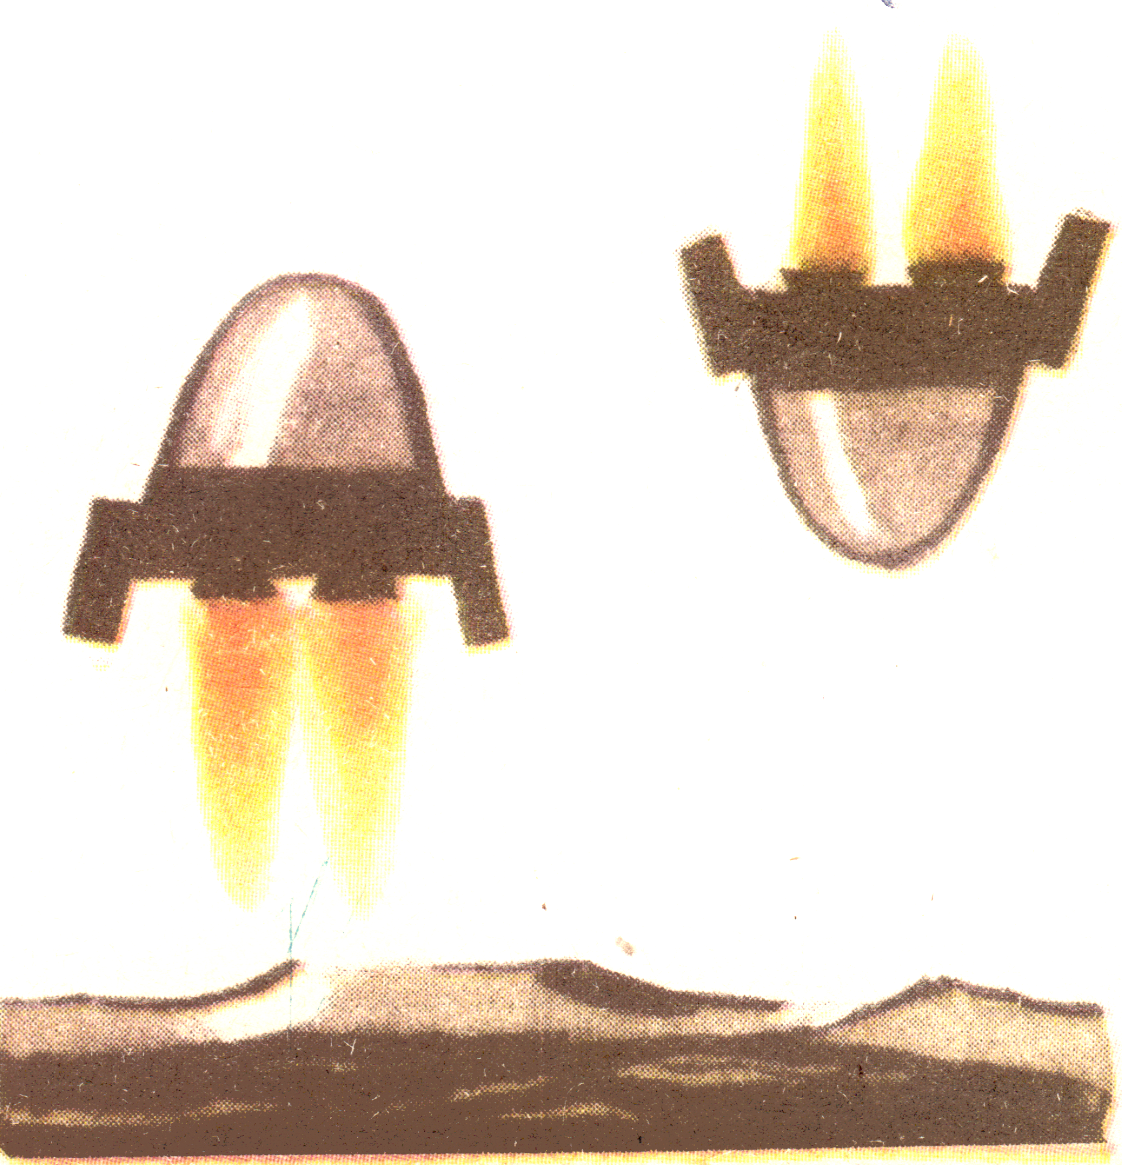
\includegraphics[width=0.5\textwidth]{lunolet1_orientation}
\caption{Нормальное торможение. Для передачи на двигатель заданного с пульта режима нужно нажать С/П (слева). Реверс тяги. Для передачи на двигатель заданного режима нажать ПП /—/ С/П (справа).}
\end{figure}

Программа «Лунолет-1» (см. стр. 52/*FIXME*/) может использоваться не только для численного моделирования маневров космических аппаратов в непосредственной близости безатмосферных небесных тел или в качестве учебного пособия, но и как основа ряда электронных игр для программируемых микрокалькуляторов. Сегодня мы знакомим читателей с одной из них. Играющий должен, регулируя тягу двигателя, посадить корабль на планету, причем скорость в момент контакта с поверхностью не должна превышать выбранного значения, например 5 м/с (мягкая посадка). Чтобы играть в эту игру, нужно после ввода программы в ПМК выполнить следующие подготовительные операции:
\begin{enumerate}
\item Сформировать и заслать в регистр 9 аварийный сигнал. Например, букву Г: Сх ÷ ВП ВП ↑ П9.
\item Ввести в память машины константы и начальные значения переменных: (ускорение свободного падения на поверхности планеты, м/с$^{2}$) П4; (масса корабля без топлива, кг) П5; (скорость истечения продуктов сгорания, м/с) П6; (предельное ускорение, которое могут выдержать космонавты, не теряя сознания, м/с$^{2}$) П7; (начальная высота, м) ПА; (начальная скорость, м/с, причем положительным считается направление вверх) ПВ; (запас топлива, кг) ПД.
\end{enumerate}

В регистре С может откладываться либо текущее время, либо время, оставшееся до установленного срока (например, если ресурс жизнеобеспечения ограничен). Для реализации первого варианта нужно набрать команду: 0 ПС 1 /—/ П0; для реализации второго: (ресурс, с) ПС 1 П0. Если же играющего время не интересует, регистры С и 0 можно не задействовать.

Все исходные данные вводятся в произвольном порядке.

Теперь нужно нажать В/О и затем С/П. Игра началась. Каждый ход можно подразделить на два этапа: анализ ситуации и ввод исходных данных для очередного маневра.

\paragraph{АНАЛИЗ СИТУАЦИИ}
При останове на экране горит значение текущей высоты полета. Командой XY на индикатор вызывается текущая скорость. После этого можно при желании вызывать из памяти любые постоянные и переменные величины (они хранятся в тех же регистрах, куда были введены соответствующие исходные данные), производить на ПМК любые расчеты. После этого можно переходить к следующему этапу.

\paragraph{ВВОД ИСХОДНЫХ ДАННЫХ ДЛЯ МАНЕВРА}

Режим двигателя при маневре определяется расходом топлива и временем, за которое этот расход произведен, и задается командой: (расход, кг) ПП (время, с). Если надо ускорить спуск, после этого отдается команда ПП /—/ (реверс тяги, см. рисунок). Реверс весьма полезен при посадках на планеты со слабой и особенно отрицательной гравитацией. Для передачи набранной команды на двигатель нужно нажать С/П и ждать появления на индикаторе очередной высоты.

Задавать время маневра равным нулю нельзя. В этом случае ускорение получилось бы бесконечно большим. Если вы ошибетесь, на экране тут же загорится прежняя высота: ПМК ждет ввода правильных данных.

\paragraph{АВАРИЙНЫЕ СИТУАЦИИ}

Если после передачи команды на двигатель на экране загорается аварийный сигнал, это означает одно из двух: либо кончилось топливо, либо ускорения превысили допустимое значение. В первом случае по завершении маневра двигатели выключатся и корабль упадет на поверхность планеты, во втором — отключатся на некоторое время (пропорциональное перегрузкам), и корабль на протяжении этого времени тоже будет свободно падать: считается, что экипаж еще не обрел способности управлять кораблем. Если был задан расход, превышающий наличный запас топлива, двигатель выключится до завершения намеченного маневра, в момент полного исчерпания топлива, причем тяга (она пропорциональна отношению расход/время) будет равна заданной.

При аварийном сигнале нужно нажать С/П. Обращаться к памяти или производить на ПМК какие-то вычисления в аварийной ситуации нельзя. Если она была связана с перегрузками, то при останове на очередной высоте в регистре 2 находится время свободного падения. Оно вызывается на индикатор командой ИП2.

Игра заканчивается, когда при очередном останове на индикаторе загорается 0 (в некоторых случаях вместо ноля может появиться небольшое положительное число, например, $1 * 10^{-5}$). Значения скорости и остальных переменных в момент посадки вызываются на индикатор теми же командами, что и в обычной ситуации. При переходе к новому варианту нужно ввести новый комплект исходных данных, причем константы, если они остались неизменными, можно не вводить. Затем нажать В/О и С/П/

Когда вы наберетесь опыта и научитесь уверенно садиться на любую планету, попытайтесь ответить на два вопроса по рассказу «Истинная правда»:
\begin{enumerate}
\item Чем можно объяснить хвастливое заявление лихого селенолога, что на посадку ему бы потребовалось меньше топлива, чем было затрачено на взлет? Какие физические явления стоят за его словами?
\item Чем принципиально отличаются ситуации, описанные на стр. 52 («Пилот, наконец, решился и нажатием кнопки отправил в реактор последние остатки топлива...») и на стр. 56 («Я повторил команду, послав в двигатель последние капли топлива...»)? Почему в первом случае у решительного пилота ничего не получится, а во втором, как мы знаем, все завершилось вполне благополучно?
\end{enumerate}

В следующем выпуске мы познакомим вас еще с несколькими электронными играми, базирующимися на программе «Лунолет-1».

\end{document}
